% Trabalho de Oficina de Política Urbana
%
% Abaixo seguem orientações originais do modelo utilizado.
%
% Siga para o conteúdo do trabalho descendo até a linha 970
%
% ==============================================================
%
% Modelo para monografia de final de curso, em conformidade
% com normas da ABNT implementadas pelo projeto abntex2.
%
% Este arquivo é fortemente baseado em exemplo distribuído no
% mesmo projeto. O projeto abntex2 pode ser acessado pela página
% http://abntex2.googlecode.com/
%
% Este arquivo pode ser rodado tanto com o pdflatex quanto com
% o lualatex.  Como contém referências bibliográficas a serem
% processadas pelo programa bibtex, este programa deve ser
% executado. Em resumo, a ordem de execução deve ser:
% rodar primeiro o pdflatex (ou o lualatex), depois o bibtex e,
% a seguir, o pdflatex (ou o lualatex ) novamente mais duas vezes,
% para assegurar que todas as referências bibliográficas e 
% citações estejam atualizadas.
%
% Para adaptar os textos para uso pessoal, usar os comandos
% imediatamente antes do \begin{document} (iniciando com o
% comando \titulo).  
%
% Este modelo está adaptado para monografias de final de curso
% em matemática da UFRJ, mas, com o uso das variáveis, pode ser
% usado para outros tipos de trabalho (mestrado, doutorado),
% outros cursos, universidades etc.  Caso a adaptação das
% variáveis não seja suficiente, pode-se alterar os comandos
% imprimircapa, imprimirfolhaderosto e imprimiraprovação, 
% fazendo as alterações necessárias.  Como os comandos definidos
% neste texto usam somente LaTeX, a sua adaptação deve ser 
% simples, bastando algum conhecimento de LaTeX.
%
% O restante do preâmbulo provavelmente  não necessitará ser
% alterado, a menos, eventualmente, das opções de chamada da
% classe abntex2, que estão definidas a seguir.
% 
\documentclass[ 
% -- opções da classe memoir que é a classe base da abntex2 --
% tamanho da fonte
12pt,
% capítulos começam em pág ímpar. Insere pág vazia, se preciso
openright,
% para imprimir uma página por folha ou visualização em video 
oneside,
% frente e verso. Margens das pag. ímpares diferem das pares.
%  twoside,
% tamanho do papel. 
a4paper,
% Caio - Ocultando bordas horríveis em hiperligações
hidelinks,
% -- opções da classe abntex2 --
% títulos de capítulos convertidos em letras maiúsculas
%  chapter=TITLE,
% títulos de seções convertidos em letras maiúsculas
%  section=TITLE,
% títulos de subseções convertidos em letras maiúsculas
%  subsection=TITLE,
% títulos de subsubseções convertidos em letras maiúsculas
%  subsubsection=TITLE,
% -- opções do pacote babel --
english,   % idioma adicional para hifenização
portuguese,   % o último idioma é o principal do documento
oldfontcommands,
]{abntex2}
%
% ==============================================================
%
% --------------------------------------------------------------
% Adicionando pacotes para recursos adicionais e defindo opções
% pertinentes
% --------------------------------------------------------------
%
% cabeçalho comum para uso com lualatex ou pdflatex
\usepackage{ifluatex}
% opções para uso com o lualatex
\ifluatex
\usepackage{fontspec}
\defaultfontfeatures{Ligatures=TeX}
% o fonte small caps é diferente no latin modern
\fontspec[SmallCapsFont={Latin Modern Roman Caps}]{Latin Modern Roman}
% pacotes da AMS 
\usepackage{amsmath,amsthm} 
% pacote para fonte específico para símbolos matemáticos
\usepackage{unicode-math}
\setmathfont{Latin Modern Math}
% latin modern tem simbolos de mathbb muito feios.
%  Trocar o fonte para estes simbolos.
\setmathfont[range=\mathbb]{Tex Gyre Pagella Math}
% opções para uso com o pdflatex
\else
\usepackage[utf8x]{inputenc}
\usepackage[T1]{fontenc}
\usepackage{lmodern}
\usepackage{etoolbox}
% pacotes da AMS 
\usepackage{amsmath,amssymb,amsthm} 
% Mapear caracteres especiais no PDF
\usepackage{cmap}
\fi

% pacotes usados tanto pelo lualatex quanto pelo pdflatex
\usepackage{lastpage}    % Usado pela Ficha catalográfica
\usepackage{indentfirst} % Indenta primeiro parágrafo 
\usepackage{color}       % Controle das cores
\usepackage{graphicx}    % Inclusão de gráficos
\usepackage{wrapfig}     % gráficos ao redor do texto
% pacote para ajustar os fontes em cada linha de forma a
% respeitar as margens
\usepackage{microtype}
% permite a gravação de texto em um arquivo indicado a partir
% deste arquivo.  Originalmente foi usado para criar o arquivo
% .bib com conteúdo de exemplo, evitando a edição de um arquivo
% .bib somente para a bibliografia
\usepackage{filecontents}

% Caio - diagramas
% http://www.texample.net/tikz/examples/smart-priority/
%\usepackage{smartdiagram}

% Caio - ladeando imagens
% https://tex.stackexchange.com/questions/57433/cannot-use-caption-under-minipage
\usepackage{caption}

% Caio - preciso de tabelas longas
% http://www.tex.ac.uk/FAQ-figurehere.html
\usepackage{longtable}

% Caio - tentando melhorar o posicionamento das imagens
\usepackage{float}

% Caio - corrigindo espaçamento conforme http://tex.stackexchange.com/questions/5683/how-to-remove-top-and-bottom-whitespace-of-longtable
\setlength{\LTpre}{0pt}
\setlength{\LTpost}{0pt}

% Caio - preciso de plotagens
%\usepackage{pgfplots}
%\pgfplotsset{compat=1.8}

% Caio - quero usar letras nas listas do enumerate conforme https://tex.stackexchange.com/questions/2291/how-do-i-change-the-enumerate-list-format-to-use-letters-instead-of-the-defaul
\usepackage{enumitem}

% Caio - modo paisagem para tabelões
\usepackage{lscape}

% Caio - adicionando o pacote hyperref
\usepackage{hyperref}
% - e definindo metadados do PDF e comportamento dos links
\hypersetup{
	%pagebackref=true,
	pdftitle={Relatório/Diagnóstico de Política Urbana}, 
	pdfauthor={Vários},
	pdfsubject={Política Urbana},
	colorlinks=false,      		% false: boxed links; true: colored links
	linkcolor=blue,          	% color of internal links
	citecolor=blue,        		% color of links to bibliography
	filecolor=magenta,      	% color of file links
	urlcolor=blue,
	bookmarksdepth=4
}

% Caio - separação silábica
%\hyphenation{}

% Caio - citações mais poderosas
%\usepackage[autostyle]{csquotes}

%-----------------------------------------------------------
%-----------------------------------------------------------
% Caio - habilitar glossário
\usepackage{glossaries}
\makeglossaries

% \newglossaryentry{ex}{name={sample},description={an example}}
\newglossaryentry{abl}{
	name={ABL},
	description={Área Bruta Locável}
}

\newglossaryentry{auj}{
	name={AUJ},
	description={Aglomeração Urbana de Jundiaí}
}

\newglossaryentry{condephaat}{
	name={CONDEPHAAT},
	description={Conselho de Defesa do Patrimônio Histórico, Arqueológico, Artístico e Turístico}
}

\newglossaryentry{cbtu}{
	name={CBTU},
	description={Companhia Brasileira de Trens Urbanos}
}

\newglossaryentry{cptm}{
	name={CPTM},
	description={Companhia Paulista de Trens Metropolitanos}
}

\newglossaryentry{spr}{
	name={SPR},
	description={São Paulo Railway Company Ltd.}
}

\newglossaryentry{efsj}{
	name={EFSJ},
	description={Estrada de Ferro Santos-Jundiaí}
}

\newglossaryentry{cmsp}{
	name={CMSP},
	description={Companhia do Metropolitano de São Paulo}
}

\newglossaryentry{embraesp}{
	name={Embraesp},
	description={Empresa Brasileira de Estudos de Patrimônio}
}

\newglossaryentry{emtu}{
	name={EMTU},
	description={Empresa Metropolitana de Transportes Urbanos de São Paulo S.A}
}

\newglossaryentry{emplasa}{
	name={Emplasa},
	description={Empresa Paulista de Planejamento Metropolitano S/A}
}

\newglossaryentry{luos}{
	name={LUOS},
	description={Lei de Uso de Ocupação do Solo}
}

\newglossaryentry{mdu}{
	name={MDU},
	description={Média por Dia Útil}
}

\newglossaryentry{ouc}{
	name={OUC},
	description={Operação Urbana Consorciada}
}

\newglossaryentry{pde}{
	name={PDE},
	description={Plano Diretor Estratégico}
}

\newglossaryentry{peuc}{name={PEUC},description={Parcelamento, Edificação e Utilização Compulsórios}}

\newglossaryentry{pl}{
	name={PL},
	description={Projeto de Lei}
}

\newglossaryentry{rmsp}{
	name={RMSP},
	description={Região Metropolitana de São Paulo}
}

\newglossaryentry{rmbs}{
	name={RMBS},
	description={Região Metropolitana da Baixada Santista}
}

\newglossaryentry{cetesb}{
	name={Cetesb},
	description={Companhia Ambiental do Estado de São Paulo}
}

\newglossaryentry{sapavel}{
	name={SAPAVEL},
	description={Sistema de Áreas Protegidas, Áreas Verdes e Espaços Livres}
}

\newglossaryentry{smdu}{
	name={SMDU},
	description={Secretaria Municipal de Desenvolvimento Urbano da Prefeitura de São Paulo}
}

\newglossaryentry{idhm}{
	name={IDHM},
	description={Índice de Desenvolvimento Humano}
}

\newglossaryentry{efs}{
	name={EFS},
	description={Estrada de Ferro Sorocabana}
}

\newglossaryentry{vlt}{
	name={VLT},
	description={Veículo Leve sobre Trilhos}
}

\newglossaryentry{brt}{
	name={BRT},
	description={Bus Rapid Transit}
}

\newglossaryentry{rffsa}{
	name={RFFSA},
	description={Rede Ferroviária Federal Sociedade Anônima}
}

\newglossaryentry{iptu}{
	name={IPTU},
	description={Imposto Predial e Territorial Urbano}
}

\newglossaryentry{fepasa}{
	name={Fepasa},
	description={Ferrovia Paulista Sociedade Anônima}
}

\newglossaryentry{iss}{
	name={ISS},
	description={Imposto Sobre Serviços de Qualquer Natureza}
}

\newglossaryentry{app}{
	name={APP},
	description={Área de Preservação Permanente}
}

\newglossaryentry{luops}{
	name={LUOPS},
	description={Legislação de Ordenamento do Uso, da Ocupação e do Parcelamento do Solo}
}

\newglossaryentry{plhis}{
	name={PLHIS},
	description={Plano Local de Habitação de Interesse Social}
}

\newglossaryentry{sabesp}{
	name={Sabesp},
	description={Companhia de Saneamento Básico do Estado de São Paulo}
}

\newglossaryentry{pddmap}{
	name={PDDMAP},
	description={Plano Diretor de Drenagem e Manejo de Águas Pluviais}
}

\newglossaryentry{agem}{
	name={AGEMBS},
	description={Agência Metropolitana da Baixada Santista}
}

\newglossaryentry{pac}{
	name={PAC},
	description={Programa de Aceleração do Crescimento}
}

\newglossaryentry{zeis}{
	name={ZEIS},
	description={Zona Especial de Interesse Social}
}

\newglossaryentry{snis}{
	name={SNIS},
	description={Sistema Nacional de Informações sobre Saneamento}
}

\newglossaryentry{fabhat}{
	name={FABHAT},
	description={Fundação Agência Bacia Hidrográfica do Alto Tietê}
}

\newglossaryentry{ipt}{
	name={IPT},
	description={Instituto de Pesquisas Tecnológicas}
}

\newglossaryentry{zczeis}{
	name={ZC-ZEIS},
	description={Zona Centralidade lindeira à ZEIS}
}

\newglossaryentry{zca}{
	name={ZCa},
	description={Zona Centralidade Ambiental}
}

\newglossaryentry{zcor1}{
	name={ZCOR-1},
	description={Zona Corredor 1}
}

\newglossaryentry{zcor2}{
	name={ZCOR-2},
	description={Zona Corredor 2}
}

\newglossaryentry{zcor3}{
	name={ZCOR-3},
	description={Zona Corredor 3}
}

\newglossaryentry{zcora}{
	name={ZCORa},
	description={Zona Corredor Ambiental}
}

\newglossaryentry{zde1}{
	name={ZDE-1},
	description={Zona de Desenvolvimento Econômico 1}
}

\newglossaryentry{zde2}{
	name={ZDE-2},
	description={Zona de Desenvolvimento Econômico 2}
}

\newglossaryentry{zeis1}{
	name={ZEIS-1},
	description={Zona Especial de Interesse Social 1}
}

\newglossaryentry{zeis2}{
	name={ZEIS-2},
	description={Zona Especial de Interesse Social 2}
}

\newglossaryentry{zeis3}{
	name={ZEIS-3},
	description={Zona Especial de Interesse Social 3}
}

\newglossaryentry{zeis4}{
	name={ZEIS-4},
	description={Zona Especial de Interesse Social 4}
}

\newglossaryentry{zeis5}{
	name={ZEIS-5},
	description={Zona Especial de Interesse Social 5}
}

\newglossaryentry{zem}{
	name={ZEM},
	description={Zona Eixo de Estruturação Transformação Metropolitana}
}

\newglossaryentry{zemp}{
	name={ZEMP},
	description={Zona Eixo de Estruturação Transformação Metropolitana Previsto}
}

\newglossaryentry{zep}{
	name={ZEP},
	description={Zona Especial de Preservação}
}

\newglossaryentry{zepam}{
	name={ZEPAM},
	description={Zona Especial de Proteção Ambiental}
}

\newglossaryentry{zer1}{
	name={ZER-1},
	description={Zona Exclusivamente Residencial 1}
}

\newglossaryentry{zer2}{
	name={ZER-2},
	description={Zona Exclusivamente Residencial 2}
}

\newglossaryentry{zera}{
	name={ZERa},
	description={Zona Exclusivamente Residencial Ambiental}
}

\newglossaryentry{zeu}{
	name={ZEU},
	description={Zona Eixo de Estruturação da Transformação Urbana}
}

\newglossaryentry{zeua}{
	name={ZEUa},
	description={Zona Eixo de Estruturação da Transformação Urbana Ambiental}
}

\newglossaryentry{zeup}{
	name={ZEUP},
	description={Zona Eixo de Estruturação da Transformação Previsto}
}

\newglossaryentry{zeupa}{
	name={ZEUPa},
	description={Zona Eixo de Estruturação da Transformação Previsto Ambiental}
}

\newglossaryentry{zm}{
	name={ZM},
	description={Zona Mista}
}

\newglossaryentry{zma}{
	name={ZMa},
	description={Zona Mista Ambiental}
}

\newglossaryentry{zmis}{
	name={ZMIS},
	description={Zona Mista de Interesse Social}
}

\newglossaryentry{zmisa}{
	name={ZMISa},
	description={Zona Mista de Interesse Social Ambiental}
}

\newglossaryentry{zoe}{
	name={ZOE},
	description={Zona de Ocupação Especial}
}

\newglossaryentry{zpds}{
	name={ZPDS},
	description={Zona de Preservação e Desenvolvimento Sustentável}
}

\newglossaryentry{zpdsr}{
	name={ZPDSr},
	description={Zona de Preservação e Desenvolvimento Sustentável da Zona Rural}
}

\newglossaryentry{zpi1}{
	name={ZPI-1},
	description={Zona Predominantemente Industrial 1}
}

\newglossaryentry{zpi2}{
	name={ZPI-2},
	description={Zona Predominantemente Industrial 1}
}

\newglossaryentry{zpr}{
	name={ZPR},
	description={Zona Predominantemente Residencial}
}

\newglossaryentry{pmsp}{
	name={PMSP},
	description={Prefeitura do Município de São Paulo}
}

\newglossaryentry{smpr}{
	name={SMPR},
	description={Secretaria Municipal de Prefeituras Regionais}
}

\newglossaryentry{smg}{
	name={SMG},
	description={Secretaria Municipal de Gestão}
}

\newglossaryentry{ibge}{
	name={IBGE},
	description={Instituto Brasileiro de Geografia e Estatística}
}

\newglossaryentry{gesp}{
	name={GESP},
	description={Governo do Estado de São Paulo}
}

%-----------------------------------------------------------
%-----------------------------------------------------------
% Comandos para definir ambientes tipo teorema em português 
\newtheorem{meuteorema}{Teorema}[chapter]
\newtheorem{meuaxioma}{Axioma}[chapter]
\newtheorem{meucorolario}{Corolário}[chapter]
\newtheorem{meulema}{Lema}[chapter]
\newtheorem{minhaproposicao}{Proposição}[chapter]
\newtheorem{minhadefinicao}{Definição}[chapter]
\newtheorem{meuexemplo}{Exemplo}[chapter]
\newtheorem{minhaobservacao}{Observação}[chapter]
%-----------------------------------------------------------
%-----------------------------------------------------------
% Pacotes de citações
\usepackage[brazilian,hyperpageref]{backref}
\usepackage[alf]{abntex2cite}   % Citações padrão ABNT
%\usepackage[num]{abntex2cite}  % Citações numéricas
% --- 
% Configurações do pacote backref
% Usado sem a opção hyperpageref de backref
\renewcommand{\backrefpagesname}{Citado na(s) página(s):~}
% Texto padrão antes do número das páginas
\renewcommand{\backref}{}
% Define os textos da citação
\renewcommand*{\backrefalt}[4]{
	\ifcase #1 %
	Nenhuma citação no texto.%
	\or
	Citado na página #2.%
	\else
	Citado #1 vezes nas páginas #2.%
	\fi}%
% --- 
% --- 
% Espaço em branco no início do parágrafo
\setlength{\parindent}{1.3cm}
% Controle do espaçamento entre um parágrafo e outro:
\setlength{\parskip}{0.2cm}  % tente também \onelineskip
% ---
% compila o indice, se este for incluído no texto
\makeindex
%
% --------------------------------------------------------- 
% ---------------------------------------------------------
% Redefinindo o comando do abntex2 para gerar uma capa  
\renewcommand{\imprimircapa}{%
	\begin{capa}
	\begin{flushleft} 
		{\Large \textsc{\imprimirinstituicao  \\
				\imprimircurso \\} }
	\end{flushleft}
	
	\vfill
	\begin{center}
		{\large \imprimirautor} \\
		{\Large \textit{\imprimirtitulo}}
	\end{center}
	
	\vfill
	\begin{center}
		{\large{\imprimirlocal \\ \imprimirano  }}
	\end{center}
	\vspace*{1cm} 
	\end{capa}
	
}

% ---------------------------------------------------------
% ---------------------------------------------------------
%
%
% ---------------------------------------------------------
% ---------------------------------------------------------
% Redefinindo o comando para gerar uma folha de rosto 
\renewcommand{\imprimirfolhaderosto}{%
	\begin{center}
		{\large \imprimirautor}
	\end{center}
	\vfill \vfill \vfill \vfill
	\begin{center}
		{\Large \textit{\imprimirtitulo}}
	\end{center}
	
	\vfill \vfill \vfill 
	\begin{flushright} 
		\parbox{0.5\linewidth}{
			\imprimirtipotrabalho\, relacionado ao 
			\imprimircurso\, da \imprimirsigla\, 
			entregue como parte do
			processo de graduação para a obtenção do 
			grau de \imprimirgrau.}
	\end{flushright} 
	
	\vfill 
	\begin{flushright} 
		\parbox{0.5\linewidth}{ \imprimirorientadorRotulo 
			\imprimirorientador\\ \imprimirttorientador}
	\end{flushright} 
	
	\ifdefvoid{\imprimircoorientador}{}{
		\begin{flushright} 
			\parbox{0.5\linewidth}{ \imprimircoorientadorRotulo 
				\imprimircoorientador\\ \imprimirttcoorientador}
		\end{flushright}
	}
	
	\vfill \vfill \vfill \vfill \vfill \vfill \vfill
	\begin{center}
		{\large{\imprimirlocal \\ \imprimirano}}
	\end{center}
	\vspace*{1cm} \newpage
}
% Final do comando para gerar uma folha de rosto 
% ---------------------------------------------------------
% ---------------------------------------------------------
%
%
% ---------------------------------------------------------
% ---------------------------------------------------------
% Definindo o comando para gerar uma folha de defesa 
\newcommand{\imprimirfolhadeaprovacao}{%
	\begin{center}
		{\large \imprimirautor}
	\end{center}
	\vfill \vfill \vfill \vfill
	\begin{center}
		{\Large \textit{\imprimirtitulo}}
	\end{center}
	
	\vfill \vfill \vfill \vfill \vfill \vfill
	\begin{flushright} 
		\parbox{0.5\linewidth}{
%			\imprimirtipotrabalho\,apresentada ao 
%			\imprimircurso\, da \imprimirsigla\, como requisito
%			para a obtenção parcial do grau de \imprimirgrau.}
		}
	\end{flushright} 
	\vfill \vfill \vfill \vfill
	Aprovada em \data.
	
	\vfill \vfill \vfill \vfill
	
	\begin{center}
		\textbf{BANCA EXAMINADORA}
		
		\vfill\vfill\vfill
		\rule{10cm}{.1pt}\\
		{\imprimirexaminadorum} \\ {\imprimirttexaminadorum}
		
		\ifdefvoid{\imprimirexaminadordois}{}{
			\vfill\vfill
			\rule{10cm}{.1pt}\\
			\imprimirexaminadordois \\ \imprimirttexaminadordois }
		
		\ifdefvoid{\imprimirexaminadortres}{}{
			\vfill\vfill
			\rule{10cm}{.1pt}\\
			\imprimirexaminadortres \\ \imprimirttexaminadortres }
		
		\ifdefvoid{\imprimirexaminadorquatro}{}{
			\vfill\vfill
			\rule{10cm}{.1pt}\\
			\imprimirexaminadorquatro \\ \imprimirttexaminadorquatro }
	\end{center}
	
	\vfill \vfill 
	\begin{center}
		{\large{\imprimirlocal \\ \imprimirano}}
	\end{center}
	\vspace*{1cm}
	\newpage
}
% Final do comando para gerar uma folha de defesa 
% ---------------------------------------------------------
% --------------------------------------------------------
%
%
%
%
%
% ---------------------------------------------------------
% --------------------------------------------------------
% definindo variáveis adicionais 
\providecommand{\imprimirsigla}{}
\newcommand{\sigla}[1]{\renewcommand{\imprimirsigla}{#1}}
%
\providecommand{\imprimircurso}{}
\newcommand{\curso}[1]{\renewcommand{\imprimircurso}{#1}}
%
\providecommand{\imprimirano}{}
\newcommand{\ano}[1]{\renewcommand{\imprimirano}{#1}}
%
\providecommand{\imprimirgrau}{}
\newcommand{\grau}[1]{\renewcommand{\imprimirgrau}{#1}}
%
\providecommand{\imprimirexaminadorum}{}
\newcommand{\examinadorum}[1]{
	\renewcommand{\imprimirexaminadorum}{#1}}
%
\providecommand{\imprimirexaminadordois}{}
\newcommand{\examinadordois}[1]{
	\renewcommand{\imprimirexaminadordois}{#1}}
%
\providecommand{\imprimirexaminadortres}{}
\newcommand{\examinadortres}[1]{
	\renewcommand{\imprimirexaminadortres}{#1}}
%
\providecommand{\imprimirexaminadorquatro}{}
\newcommand{\examinadorquatro}[1]{
	\renewcommand{\imprimirexaminadorquatro}{#1}}
%
\providecommand{\imprimirttorientador}{}
\newcommand{\ttorientador}[1]{
	\renewcommand{\imprimirttorientador}{#1}} 
%
\providecommand{\imprimirttcoorientador}{}
\newcommand{\ttcoorientador}[1]{
	\renewcommand{\imprimirttcoorientador}{#1}}
%
\providecommand{\imprimirttexaminadorum}{}
\newcommand{\ttexaminadorum}[1]{
	\renewcommand{\imprimirttexaminadorum}{#1}}
%
\providecommand{\imprimirttexaminadordois}{}
\newcommand{\ttexaminadordois}[1]{\renewcommand{
		\imprimirttexaminadordois}{#1}}
%
\providecommand{\imprimirttexaminadortres}{}
\newcommand{\ttexaminadortres}[1]{
	\renewcommand{\imprimirttexaminadortres}{#1}}
%
\providecommand{\imprimirttexaminadorquatro}{}
\newcommand{\ttexaminadorquatro}[1]{
	\renewcommand{\imprimirttexaminadorquatro}{#1}}
% fim da definição de variáveis adicionais
% ---------------------------------------------------------
% ---------------------------------------------------------
%
% ---
% ---
% ---
% ---
% ---
% ---
% ---
% ---
% ---
% Informações de dados para CAPA, FOLHA DE ROSTO e FOLHA DE DEFESA
%
%----------------- Título e Dados do Autor -----------------
\titulo{Diagnóstico \& Proposta}
\autor{Bruna Fernandes \and
	   Caio César C. Ortega \and
	   Jade Vieira Cavalhieri \and
	   Leonardo Barbosa \and
	   Luciana Akemi
}
%

%----------Informações sobre a Instituição e curso -----------------
\instituicao{Universidade Federal do ABC \\
	Centro de Engenharia, Modelagem e Ciências Sociais Aplicadas}
%
\sigla{UFABC}
%
\curso{Bacharelado em Planejamento Territorial}
%\curso{Curso de Licenciatura em Matemática}
%\curso{Mestrado em Ensino de Matemática}
%\curso{Doutorado em Matemática}
%
\local{São Bernardo do Campo, SP}
%
%
% -------- Informações sobre o tipo de documento
\tipotrabalho{Relatório}
%\tipotrabalho{Monografia de final de curso}
%\tipotrabalho{Dissertação de mestrado}
%\tipotrabalho{Tese de doutorado}
%
\grau{BACHAREL em Planejamento Territorial}
%\grau{LICENCIADO em Matemática}
%\grau{MESTRE em Matemática}
%\grau{DOUTOR em Ciências}
%
\ano{2018}
\data{13 de Junho de 2018} % data da aprovação
%
%------Nomes do Orientador, examinadores.  
\orientador{Érico R. P. Novais}
%\coorientador{Antonio da Silva} % opcional
\examinadorum{Érico R. P. Novais}
%\examinadordois{Ivo Fernandez Lopez}
%\examinadortres{Jeferson Leandro Garcia de Araújo}
%\examinadorquatro{Antonio da Silva}
%
%--------- Títulos do Orientador e examinadores ----
%\ttorientador{Bacharel em Física - UEFS}
%\ttcoorientador{Doutor em Matemática - UFRJ} 
%\ttexaminadorum{Doutor em Matemática - UFRJ}
%\ttexaminadordois{Doutor em Matemática - UFRJ}
%\ttexaminadortres{Doutor em Matemática - UFRJ}
%\ttexaminadorquatro{Doutor em Matemática - UFRJ}
%
% ---
% ---
\begin{document}
		
	% ---
	% Chamando o comando para imprimir a capa
	\imprimircapa
	% ---
	% ---
	% Chamando o comando para imprimir a folha de rosto
	%\imprimirfolhaderosto
	% ---
	% ---
	% Chamando o comando para imprimir a folha de aprovação
	%\imprimirfolhadeaprovacao
	% ---
	% ---
	% Dedicatória
	% ---
	%	\begin{dedicatoria}
	%  	 \vspace*{\fill}
	%  	 \centering
	%  	 \noindent
	%  	 \textit{ Este trabalho é dedicado a todos que, com entusiasmo,\\
	%  	 		sonham e lutam por XYZ no ABCDEFG\\
	%  			do XPTO.} \vspace*{\fill}
	%	\end{dedicatoria}
	%	
	%	
	%	\begin{agradecimentos}
	%	Orientação do modelo: insira aqui um parágrafo
	%	\end{agradecimentos}
	%	
	%	
	%
	%---------------------- EPÍGRAFE I (OPCIONAL)--------------
	%\begin{epigrafe}
	%    \vspace*{\fill}
	%    \begin{flushright}
	%        \textit{''Texto''\\
	%        Autor}
	%    \end{flushright}
	%\end{epigrafe}
	%
	%
	%
	%--------Digite aqui o seu resumo em %Português--------------
	%\begin{resumo}
	%   Descrição. 
	%
	%   \vspace{\onelineskip}
	%   \noindent
	%   \textbf{Palavras-chaves}: Palavras.
	%\end{resumo}
	
	
	%
	% --- resumo em inglês (abstract) ---
	%\begin{resumo}[Abstract]
	%   \begin{otherlanguage*}{english}
	%      Description.
	%
	%      \vspace{\onelineskip}
	%      \noindent
	%      \textbf{Keywords}: Words.
	%   \end{otherlanguage*}
	%\end{resumo}

	%
	%----Sumário, lista de figuras e lista de tabelas ------------
	\tableofcontents 
	\newpage \listoffigures
	\newpage \listoftables
	%---------------------
	%--------------Início do Conteúdo---------------------------
	% o comando textual é obrigatório e marca o ponto onde começa 
	% a imprimir o número da página
	\textual
	%
	%---------------------
	%


%
% O conteúdo começa pra valer a seguir
%

%
%===============================================================================
%
	
	\chapter{Introdução}

	O município de Francisco Morato foi selecionado como objeto de estudos para a disciplina, representando um misto de desafio e oportunidade de aprendizado. Para encarar o município, lançamos mão não só do arcabouço teórico estudado na disciplina de Política Urbana, mas também das abordagens práticas da própria disciplina de Oficina de Política Urbana. Quando apropriado, outras fontes secundárias também foram utilizadas. Como o intuito de tornar a proposta assertiva, realizamos um diagnóstico do município.
	
	\chapter{Trajetória de Francisco Morato}
	% Item 1 da metodologia adotada:
	% Quais são as grandes etapas já experimentadas pelo território ao longo de sua história?
	
	O capítulo sumariza as grandes etapas que o território já experimentou ao longo de sua história.
	
	\section{As grandes etapas}
	
	As grandes etapas são as seguintes, sumarizadas na lista abaixo e na figura \ref{fig:timeline}, sendo que a emancipação de Francisco Morato está contextualizada no mapa da figura \ref{spmetrop_pag046}.
	
	\begin{itemize}
		\item Construção da linha ferroviária pela \gls{spr} em 1867 \cite[p.26]{ferreira2010a};
		\item Elevação de Franco da Rocha à categoria de município em 30/11/1944 \cite{ibge2018a};
		\item Povoamento do distrito de Francisco Morato a partir do loteamento da Fazenda Belém \cite[p.57]{cassiele2007a};
		\item Emancipação do distrito de Francisco Morato de Franco de Rocha em 28/02/1964 \cite[p.57]{cassiele2007a}.
	\end{itemize}
	
	\begin{figure}[H]
		\centering
		\caption[Diagrama do surgimento de Francisco Morato]{Breve diagrama de eventos que desencadearam no surgimento de Francisco Morato}
		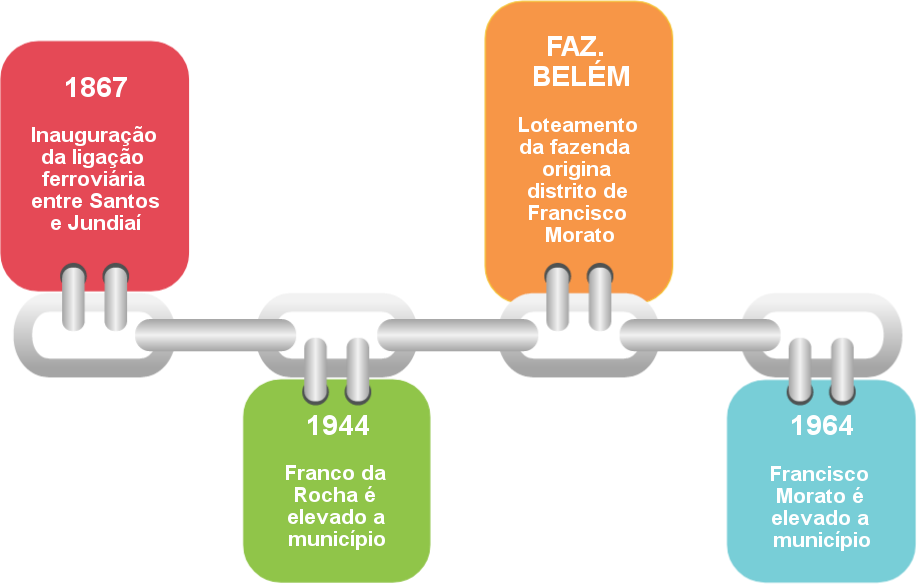
\includegraphics[height=8cm]{img/linha_do_tempo}
		\label{fig:timeline}
		\legend{Fonte: elaboração própria}
	\end{figure}
	
	\begin{figure}[h]
		\centering
		\caption{Desmembramentos de municípios metropolitanos 1940 a 2000}
		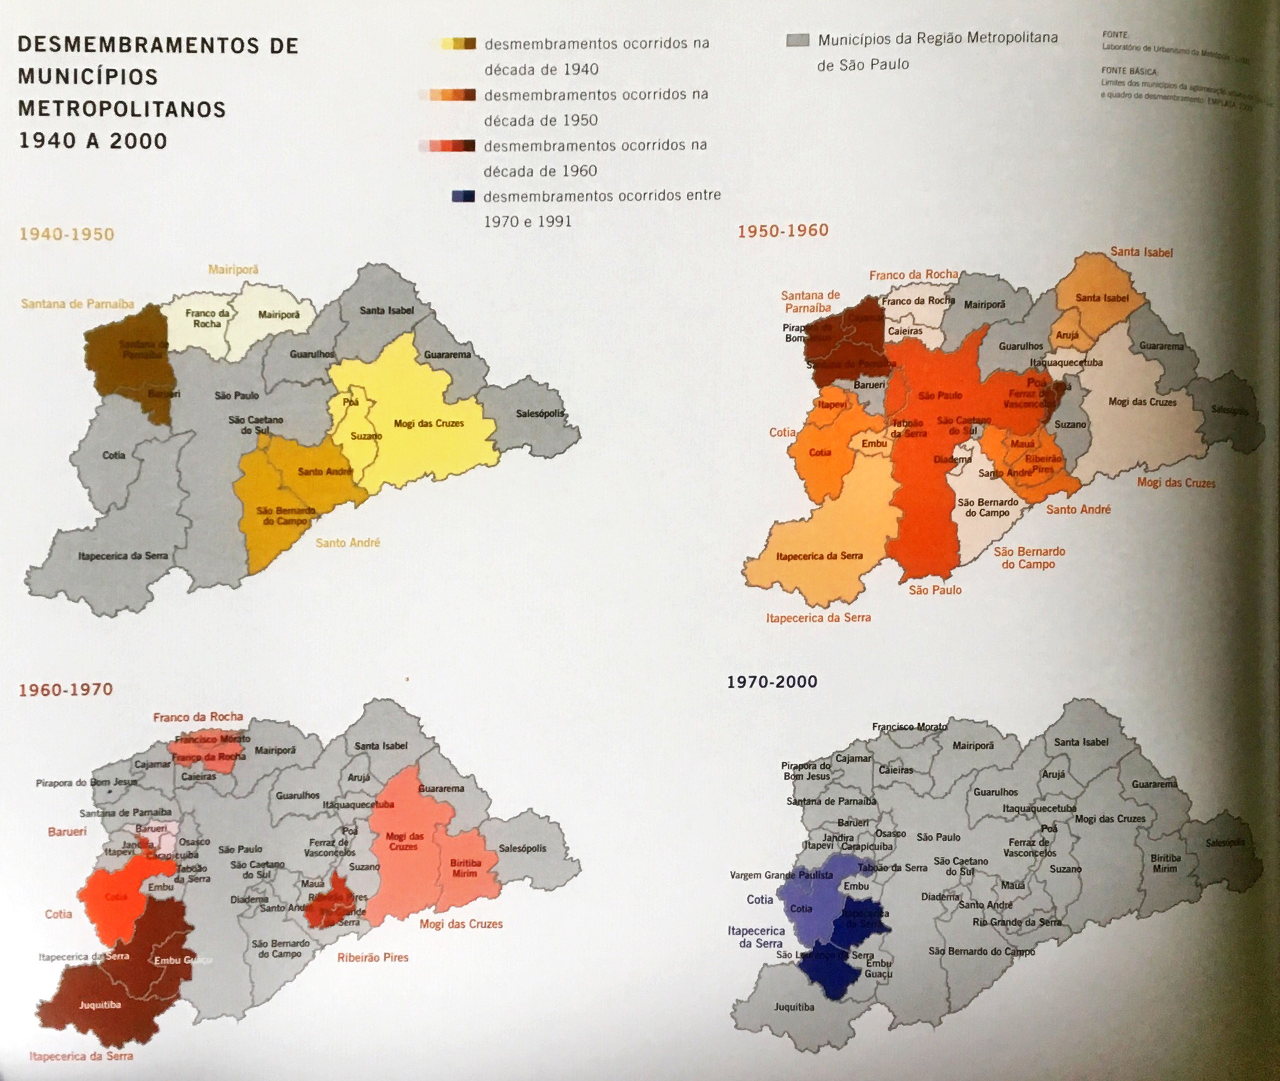
\includegraphics[width=\linewidth,keepaspectratio]{img/spmetrop_pag046}
		\label{spmetrop_pag046}
		\legend{Elaboração por \citeonline[p.46]{meyer2004}}
	\end{figure}
	
	\section{Compreendendo a trajetória} \label{sec:balanco}
	% Item 3 da metodologia adotada:
	% Quais são os pontos fracos e fortes (consequências para o território) que aparecem nesta trajetória?
	%
	
	São os aspectos-chave: 
	
	\begin{itemize}
		\item Migração nordestina;
		\item Mão de obra barata;
		\item Manutenção da segregação;
		\item Altos índices de pendularidade;
		\item Negligência institucional.
	\end{itemize}
	
	\subsection{Caracterização do tecido}
	
	Conforme \citeonline[p.64]{cptm2010a} (grifo nosso), ``a Linha 7 faz parte do sistema construído no final do Século XIX pela São Paulo Railway Company Ltd. (\gls{spr}), mais tarde \gls{efsj} – Estrada de Ferro Santos-Jundiaí. O serviço de trens de subúrbio começou no início do século XX, inicialmente até Pirituba. Diferentemente da Linha 10, que também faz parte do mesmo sistema da SPR, \textbf{essa linha teve uma importância menor na instalação de indústrias ao longo de seu traçado devido, provavelmente, ao seu fator geográfico}''.
	
	% O trabalho de Rosa, citado abaixo, realiza uma série de análises a partir da OD 1997 utilizando Francisco Morato como objeto de estudo, incluindo mapas plotados para espacializar os comportamentos observados. Vale a pena dar uma olhada no PDF da tese.
	
	\citeonline[p.116]{rosa2006a} constrói um panorama do município em 2006 a partir da Associação Cultural Comunitária Pró-Morato, no qual se destacam a pobreza, a precariedade e o desemprego, incluindo a baixa possibilidade de empregabilidade dentro do município:
	
	\begin{citacao}
		Segundo a Associação Cultural Comunitária Pró-Morato (2006), o baixo poder aquisitivo da população, o desemprego, a precariedade dos serviços públicos, a falta de espaços para lazer, cultura, esportes, educação e capacitação profissional concede ao município o maior índice de exclusão social da \gls{rmsp}. Sua estrutura comercial e industrial é insuficiente para absorver a mão-de-obra residente na cidade, fazendo com que seus moradores busquem trabalho na capital ou região, sendo considerada cidade-dormitório.
	\end{citacao}
	
	Tratam-se de características que também foram observadas por \citeonline[p.70]{cptm2010a}, que aponta que Francisco Morato ``apresenta altas taxas de crescimento demográfico,	baixa concentração de empregos, renda média familiar baixa e um grande movimento pendular nos fluxos matinais e vespertinos do sistema ferroviário'', também descrevendo a área central, na qual a estação homônima (e a única que atende ao município) está presente como sendo ``típica de subúrbio metropolitano, com o uso predominante do solo essencialmente comercial, de caráter popular, na margem oeste da ferrovia, e habitacional de baixa densidade e baixa renda na margem leste'', apontando ainda que Francisco Morato ``apresenta uma vasta e densa rede hídrica que causa problemas de alagamento na linha férrea e cria restrições para a ocupação urbana'', traço último este que será especialmente considerado para a elaboração da proposta de lei, que visará minimizar impactos, ainda que preveja a qualificação de parcelas do território, com vistas à redução da pendularidade. \citeonline[p.60]{suarez2014a} classifica Francisco Morato entre os ``núcleos que já nasceram como subúrbios, muitas vezes tendo se formado a partir de uma estação ferroviária'' para qualificar o processo de conurbação da região.
	
	\begin{figure}[h]
		\centering
		\caption{Conjuntos habitacionais de interesse social na \gls{rmsp}}
		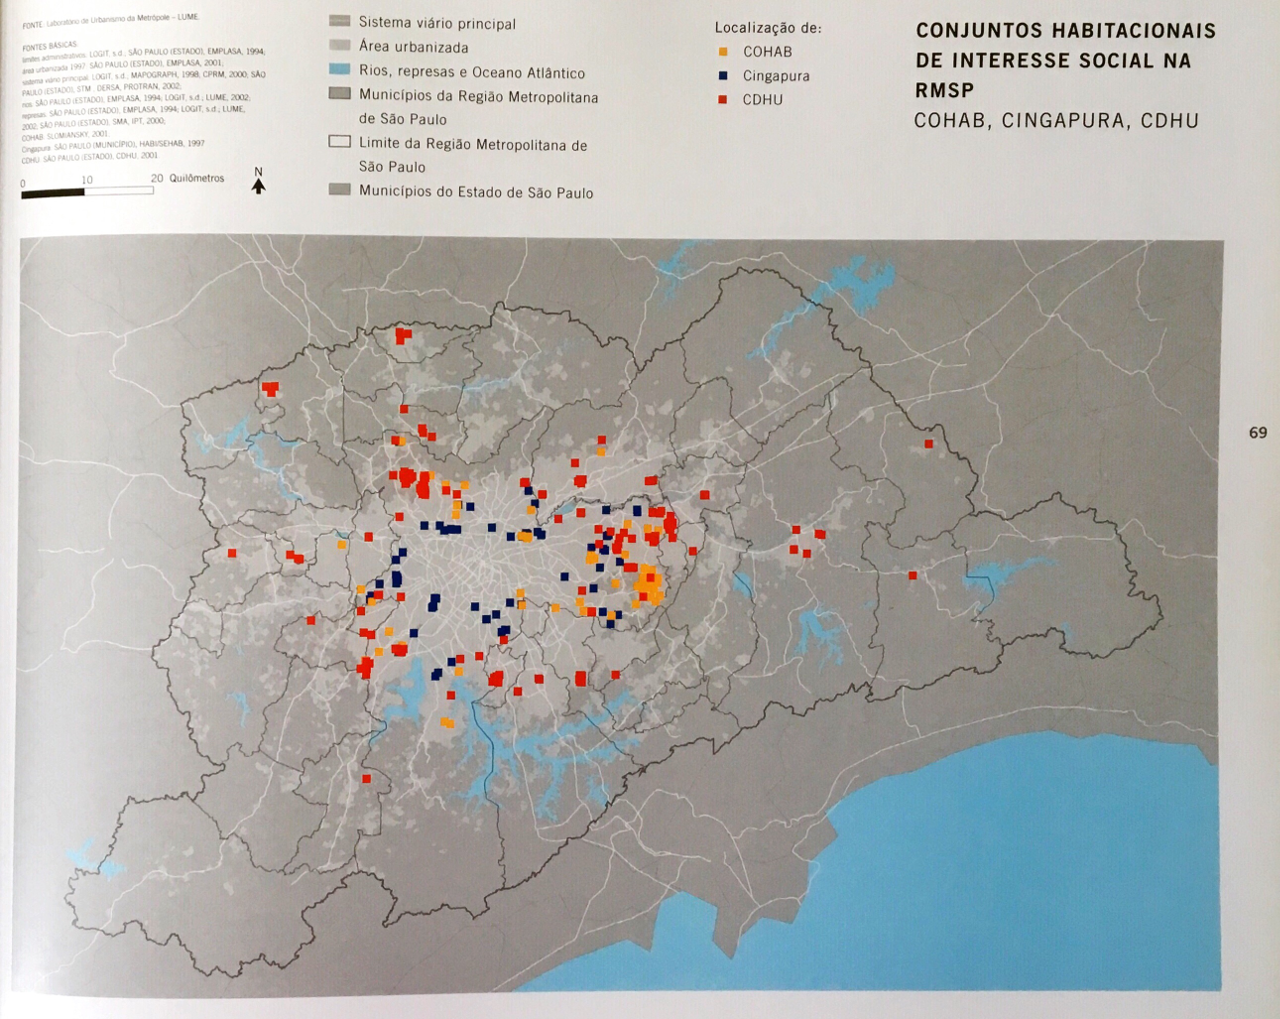
\includegraphics[width=\linewidth,keepaspectratio]{img/spmetrop_pag069}
		\label{spmetrop_pag069}
		\legend{Elaboração por \citeonline[p.69]{meyer2004}}
	\end{figure}

	\begin{figure}[h]
		\centering
		\caption{Padrões de renda e habitação própria na \gls{rmsp} - 1991 a 2000}
		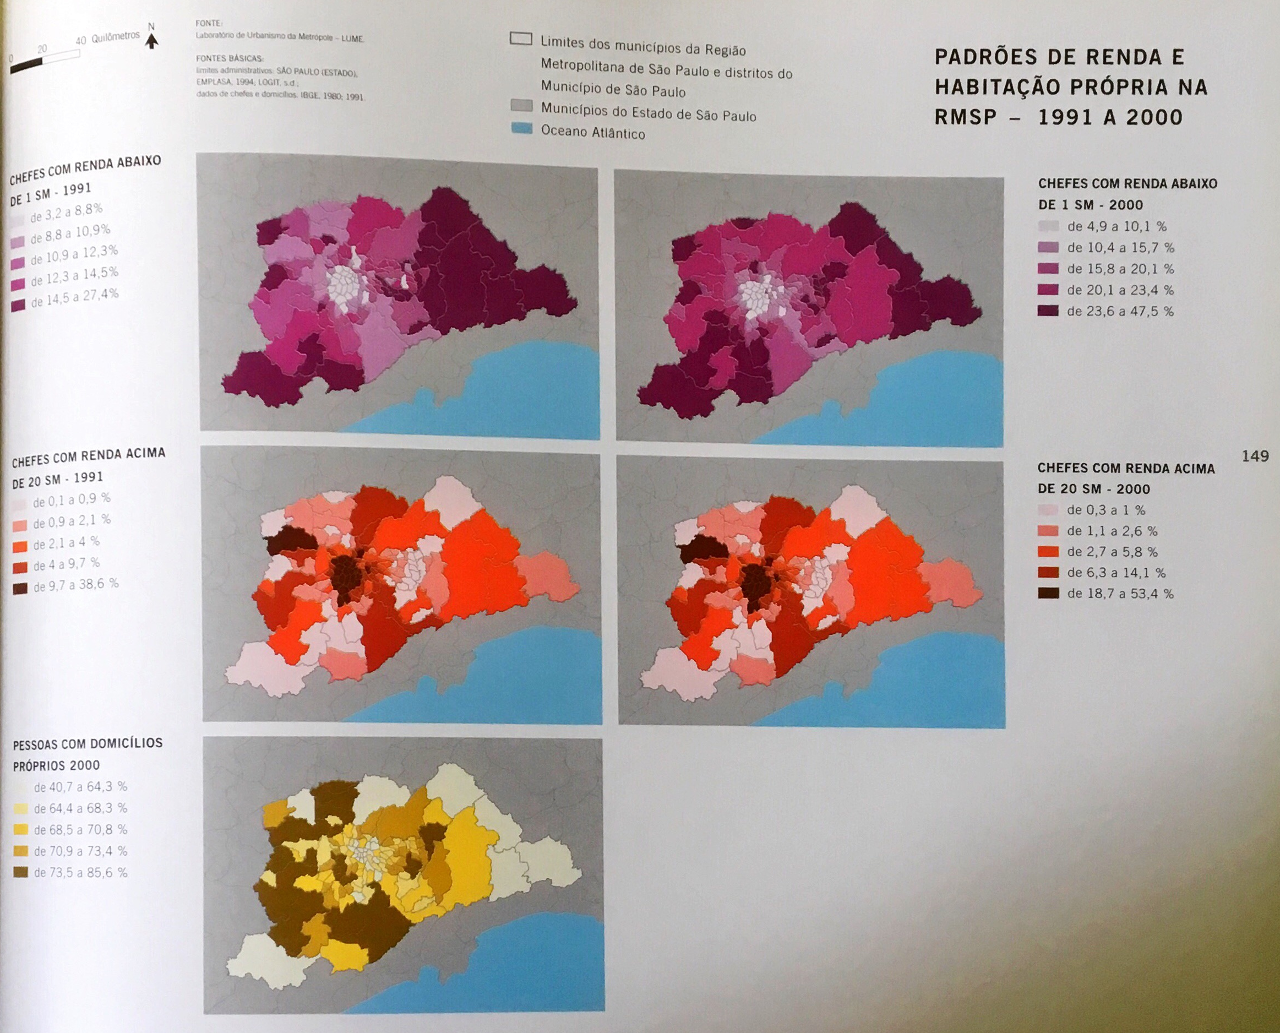
\includegraphics[width=\linewidth,keepaspectratio]{img/spmetrop_pag149}
		\label{spmetrop_pag149}
		\legend{Elaboração por \citeonline[p.149]{meyer2004}}
	\end{figure}
	
	Quanto ao uso habitacional descrito, é oportuna a crítica sintetizada por \citeonline[p.22]{cassiele2007a}: ``a política do Laissez-Faire urbano favoreceu os especuladores imobiliários e a explosão do número de loteamentos clandestinos na periferia paulistana. A justificativa da política era buscar o alívio à crise de escassez de moradias'', sendo que, para \citeonline[p.13]{villaca1986a}, a moradia ideal é aquela ``que a classe trabalhadora acha que pode conquistar através do avanço possível dentro das condições políticas, sociais e econômicas em que se encontra'', no entanto, o desenvolvimento econômico do país não tem, necessariamente, significado melhorias substanciais na condição de vida do proletariado, assim ``não há como negar que as condições de vida da maioria do povo brasileiro são aterradoramente baixas'' \cite[p.14]{villaca1986a}, bem como que ``a transformação da habitação em `casa própria' é uma necessidade histórica do capitalismo'' \cite[p.19]{villaca1986a}, transformando a habitação em mercadoria, ainda que repleta de especificidades, o que resulta, por exemplo, no oferecimento de financiamentos. A casa própria então pode ser produzida para a classe média ou ser autoconstruída, sendo que a autoconstrução dialoga com a facilidade de exploração da classe trabalhadora, que chega a viver com condições urbanas e habitacionais ``rebaixadas a níveis medievais'' \cite[p.21]{villaca1986a}. Villaça também aponta que há ainda uma parcela mais pobre da classe trabalhadora, que não consegue adquirir material de construção novo e terrenos, o que resulta no uso de material de construção velho, usado ou adaptado, além da invasão de terrenos públicos, privados ou em condição subótima (alagados e encostas, por exemplo). Diante de um quadro tão precário, começam a surgir loteamentos populares, que ainda que fossem clandestinos, eram tolerados pelo poder público, reforçando uma dicotomia na produção da cidade, mantendo a classe operária afastada da burguesia. Nos loteamentos populares a autoconstrução era regra. No Nordeste a invasão predominou sobre os loteamentos. A casa própria começa no plano ideológico e transita para o plano da realidade: ``hoje, a importância da casa própria está longe de ser ideológica. Corresponde a relações reais. A posse de uma casa não só confere mais status como facilita as relações econômicas, abre as portas aos empréstimos e aos crediários e constitui não só uma forma bastante segura de investimento como uma eficaz defesa contra a inflação'' \cite[p.24]{villaca1986a}.
	
	\citeonline[p.59]{cassiele2007a} aponta que ``em Francisco Morato a auto-construção persiste ainda hoje, apesar de ser bem menos intensa do que nas décadas de 50 a 80. Há ainda a venda de lotes a preços acessíveis à classe trabalhadora de baixa renda''.
	
	\begin{figure}
		\caption{Conjunto habitacional e loteamento popular em Francisco Morato}
		\begin{minipage}{.5\linewidth}
			\centering
			\subfloat{\label{spmetrop_pag256:a}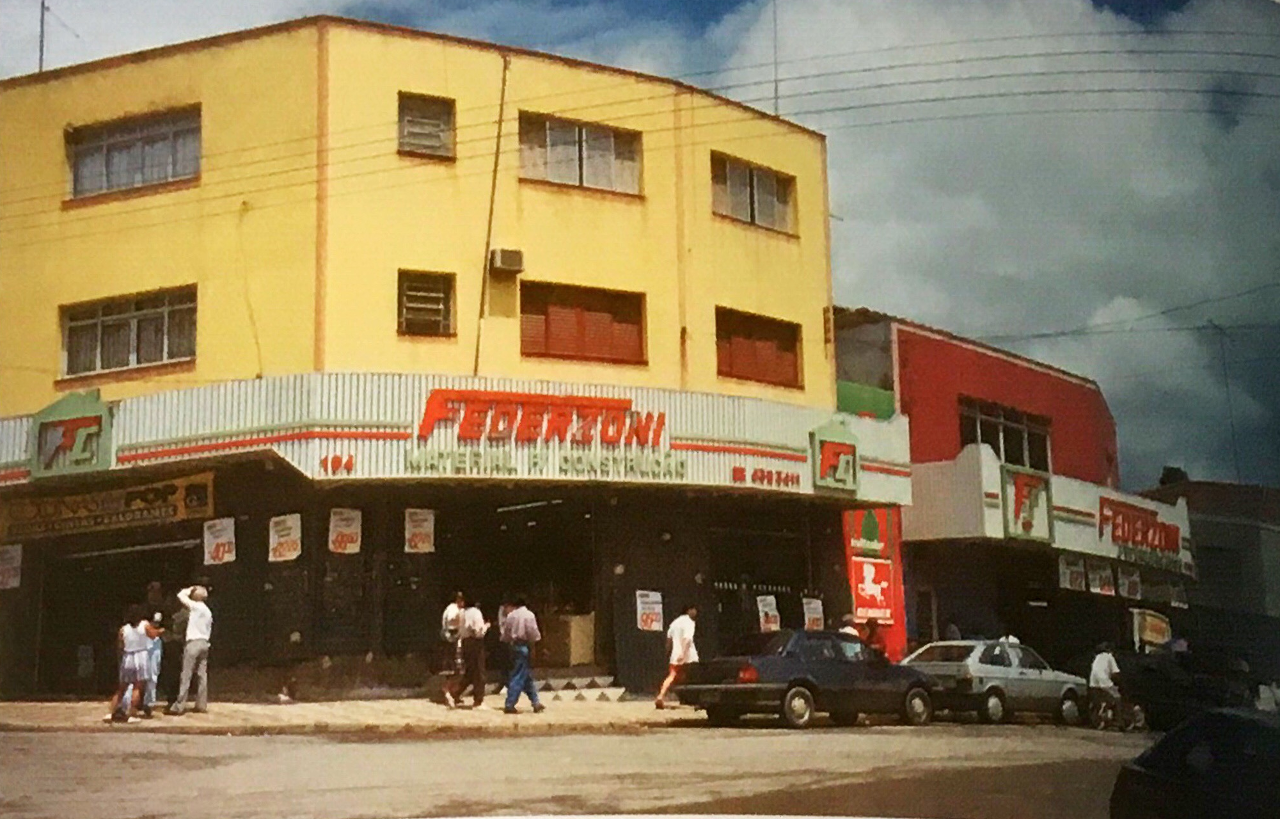
\includegraphics[height=4cm,keepaspectratio]{img/spmetrop_pag256a.png}}
		\end{minipage}%
		\begin{minipage}{.5\linewidth}
			\centering
			\subfloat{\label{spmetrop_pag256:b}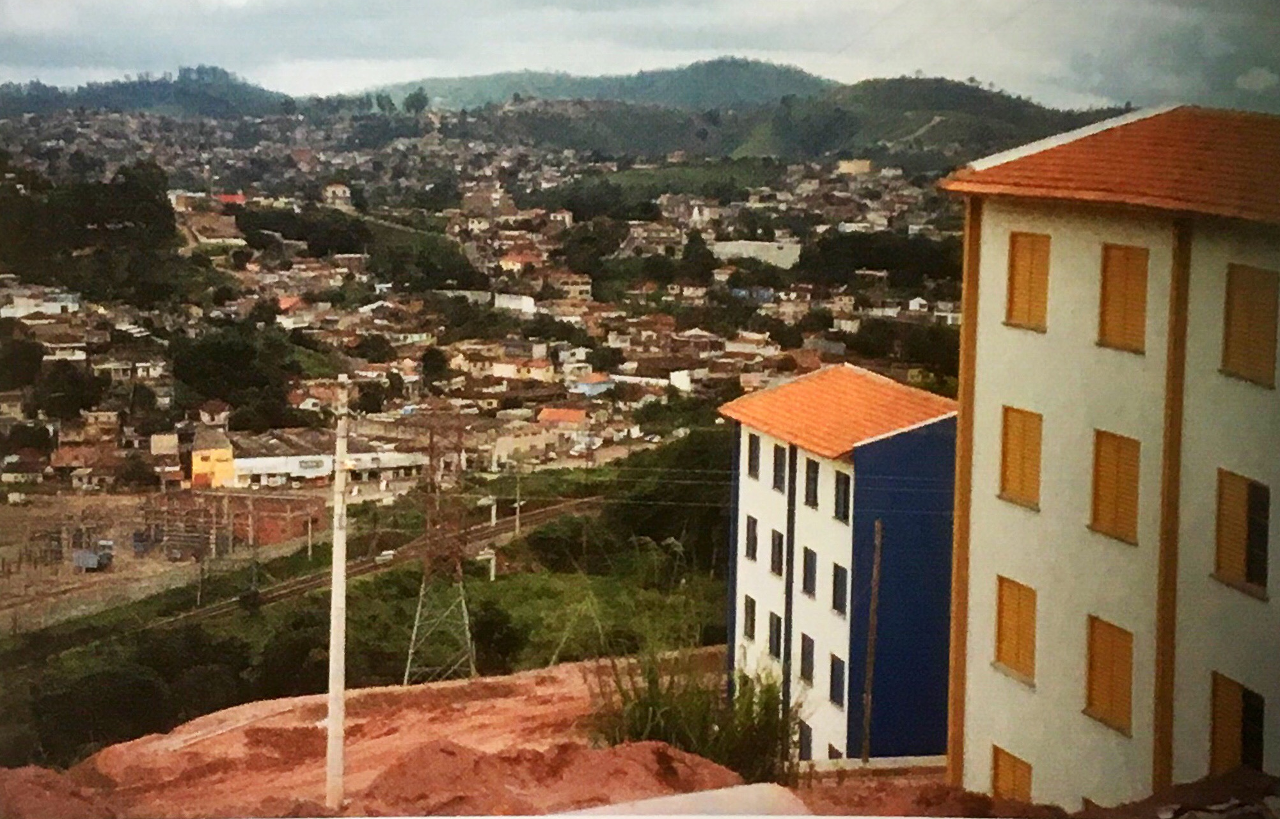
\includegraphics[height=4cm,keepaspectratio]{img/spmetrop_pag256b.png}}
		\end{minipage}\par\medskip
			\centering
			\subfloat{\label{spmetrop_pag256:c}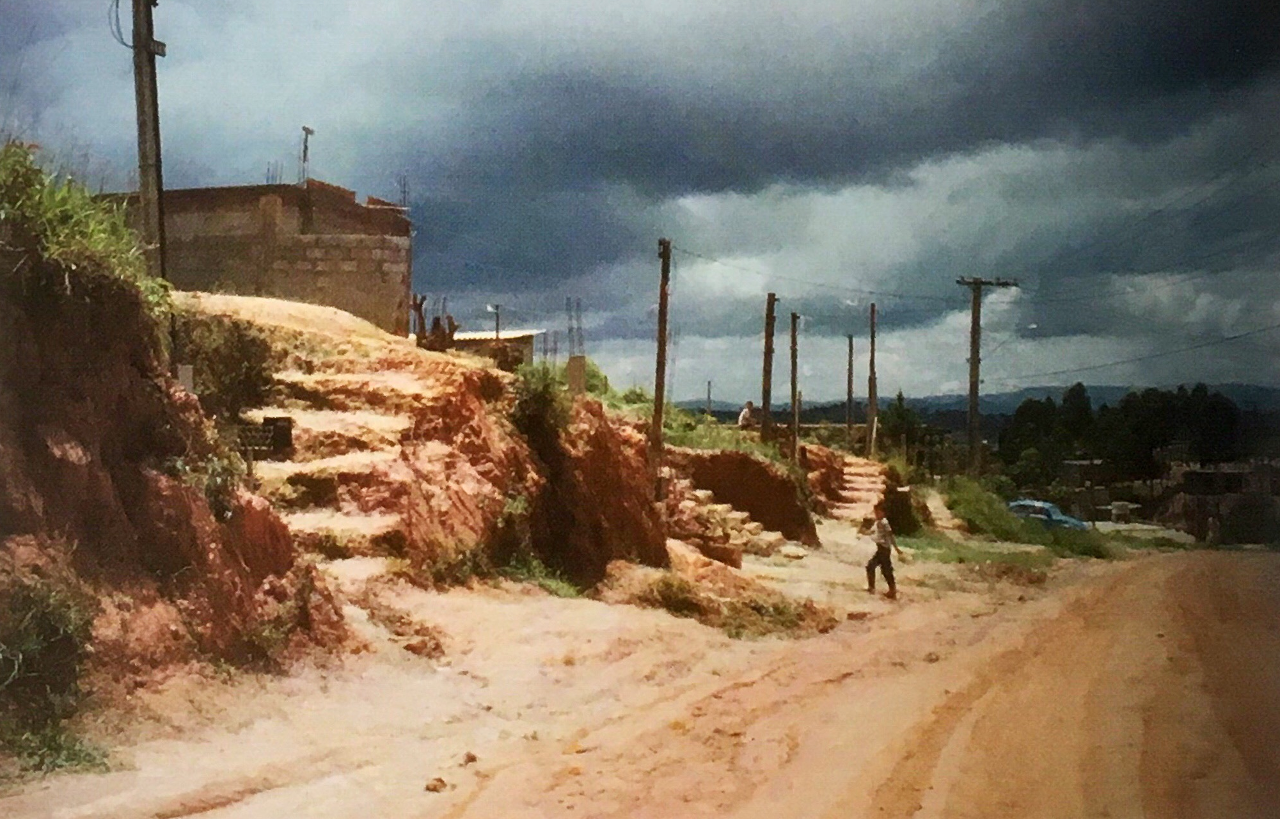
\includegraphics[height=4cm,keepaspectratio]{img/spmetrop_pag256c.png}}
		\label{fig:spmetrop_pag256}
		\legend{Fonte: \citeonline[p.256]{meyer2004}}
	\end{figure}
	
	A questão habitacional também esbarra em outro aspecto do capitalismo: a construção da acessibilidade, a noção de ``perto'', ``longe'' e ``fora de mão'' para (des)qualificar determinadas localidades. \citeonline[p.38]{villaca1986a} salienta que ``a casa tende cada vez mais e para crescentes parcelas da população, a se reduzir a local de repouso'', pois a cidade se torna o local de viver, já que também é o local de reprodução da força de trabalho. As relações pré-capitalistas, quando a casa abrigava diferentes utilizações e sociabilidades, são desfeitas, externadas para a cidade. Existe, portanto, uma disputa entre classes sociais quanto à produção do espaço urbano, já que o tempo não pode ser controlado diretamente e é refém dos deslocamentos intraurbanos. Tal fenômeno, como discorre \citeonline[p.42]{villaca1986a}, vai resultar na produção de novos centros e na rejeição dos centros ocupados pelas classes populares, o que se dá, por exemplo, com a fuga de famílias e empreendimentos das classes médias e altas para se encaixarem nos novos centros produzidos, empobrecendo o comércio e população dos bairros afetados.
	
	\subsection{Crescimento e migração} \label{CrescimentoMigracao}
	
	Para iniciar esta subseção, valemo-nos da obra de \citeonline[p.42]{meyer2004}, a qual aponta que ``a relação entre a expansão da mancha urbana, desenvolvimento econômico e crescimento populacional introduz elementos importantes para a compreensão dos processos urbanos'', assim sendo, recuperamos que, conforme \apudonline[p.41]{langenbuch1968}{meyer2004} ``no período 1940-1960, enquanto a cidade central, o trecho dito urbano da metrópole, apresentava sua população aumentada em 171\%, os seus arredores cresciam 364\%''. Entre 1960 e 1970 o ganho migratório na \glsdesc{rmsp} foi de aproximadamente 2 milhões de pessoas, atraídas pelo mercado de trabalho expandido, com ocupações tanto industriais quanto no setor de serviços \cite[p.42]{meyer2004}.
	
	Conforme \citeonline[p.65]{cassiele2007a} ``na década de 70 Francisco Morato, assim como toda a periferia paulistana recebeu grande contingente populacional que buscava lotes baratos e com pagamento facilitado para então construírem suas moradias'', apontando, com base em sua pesquisa de campo, também que ``a cidade é formada em grande parte por migrantes de diversas partes do país, principalmente nordestinos, que se mudaram de sua terra natal para São Paulo'', escolhendo Francisco Morato para a  construção da unidade habitacional, ``pois os preços dos terrenos próximos à metrópole eram incompatíveis com seu poder de compra'' \citeonline[p.57]{cassiele2007a}.

	\begin{figure}[h]
		\centering
		\caption{Evolução da população e taxa de crescimento populacional por subregiões da \gls{rmsp} 1970 a 2000}
		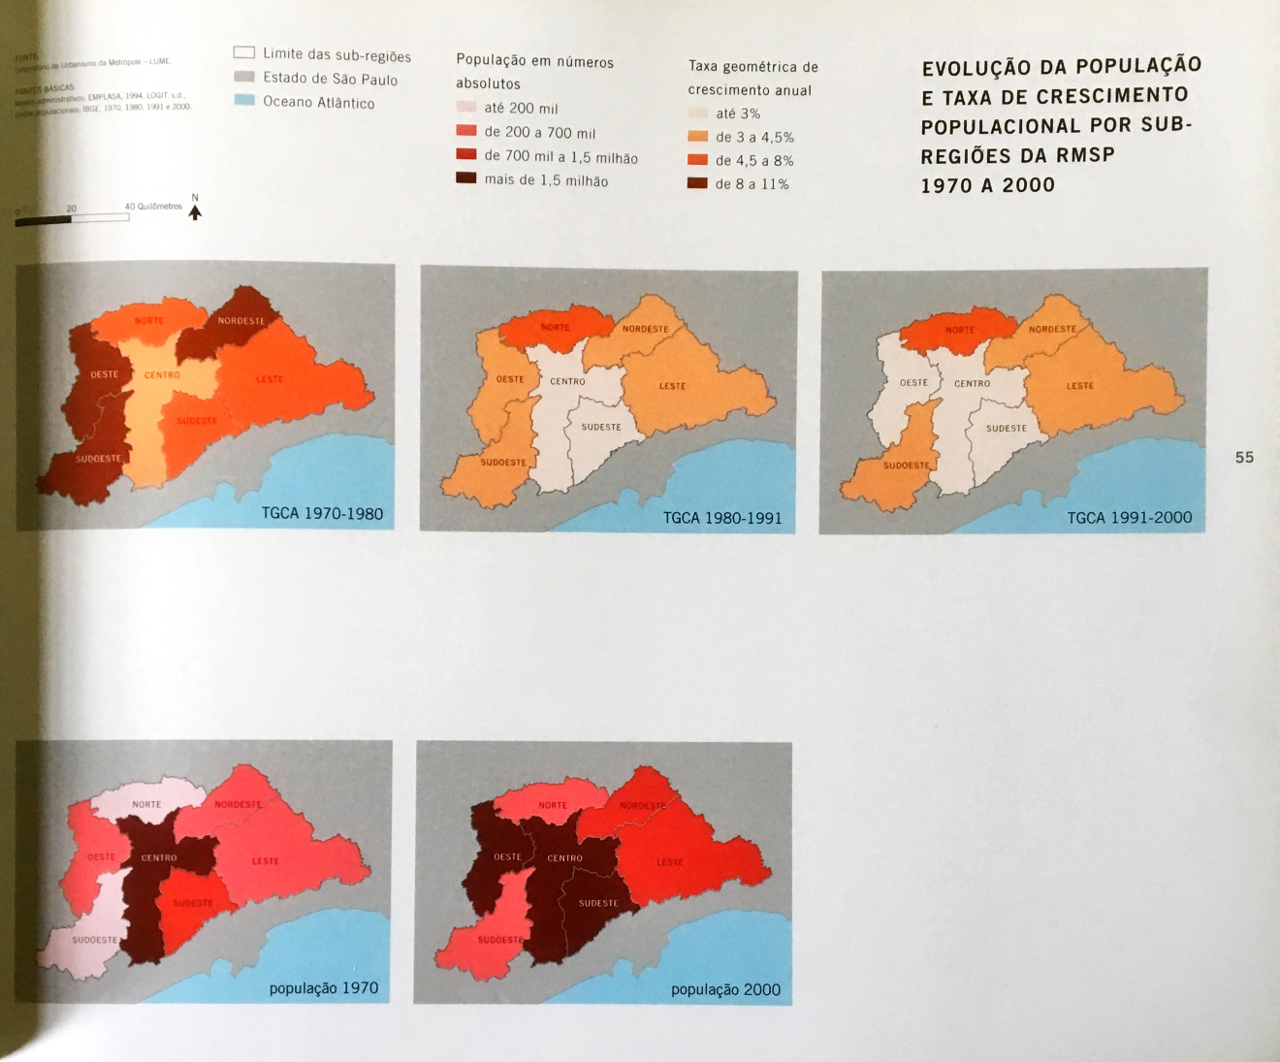
\includegraphics[width=\linewidth,keepaspectratio]{img/spmetrop_pag055}
		\label{spmetrop_pag055}
		\legend{Elaboração por \citeonline[p.55]{meyer2004}}
	\end{figure}
	
	\begin{figure}[h]
		\centering
		\caption{Evolução da taxa de crescimento populacional na \gls{rmsp} 1950 a 2000 }
		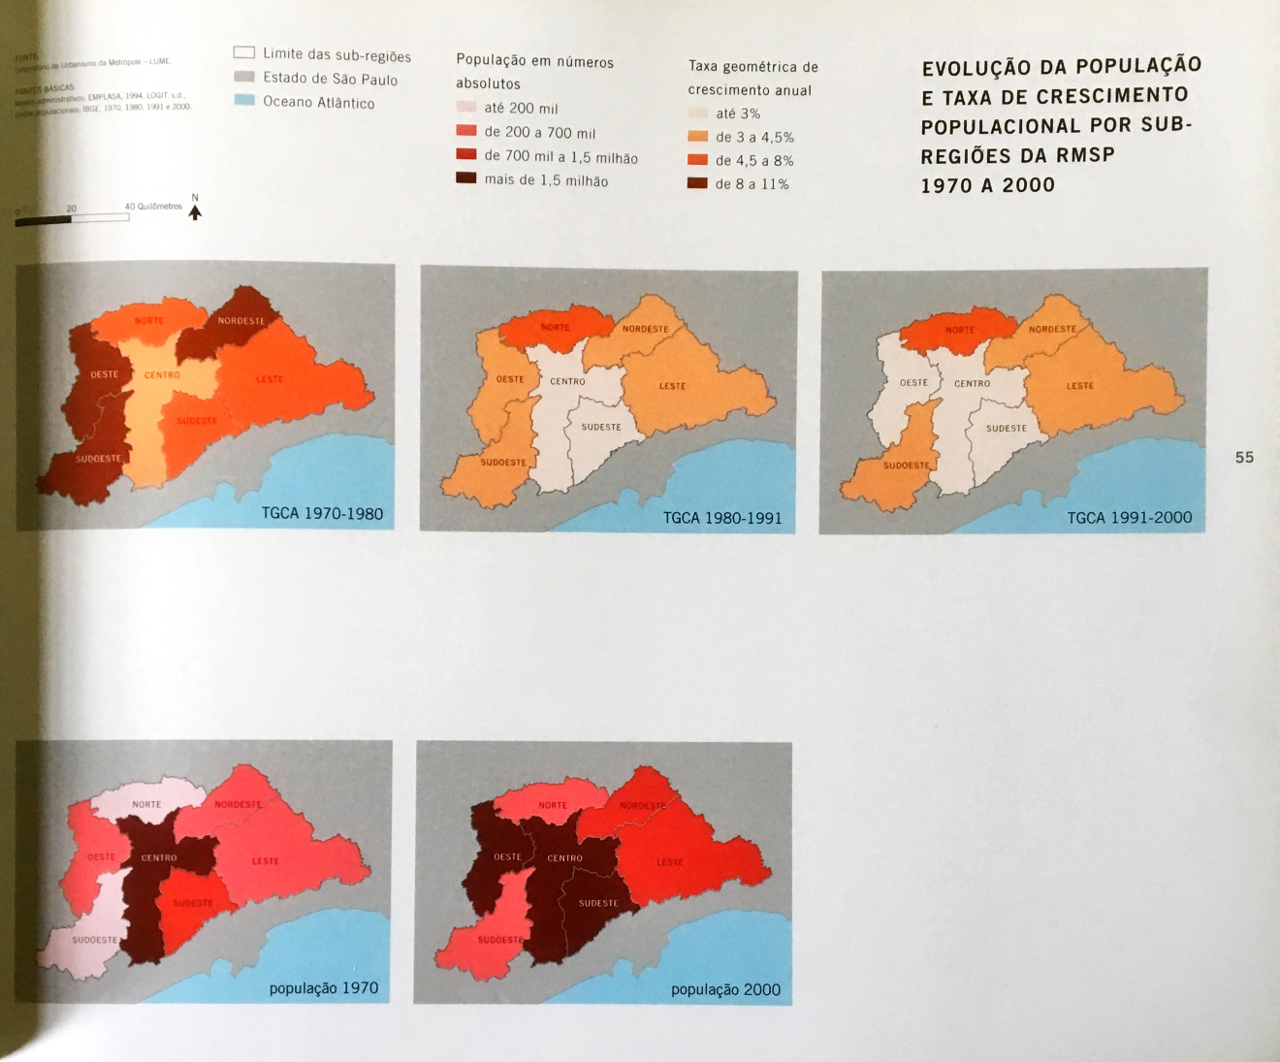
\includegraphics[width=\linewidth,keepaspectratio]{img/spmetrop_pag055}
		\label{spmetrop_pag060}
		\legend{Elaboração por \citeonline[p.60]{meyer2004}}
	\end{figure}
	
	\begin{figure}[h]
		\centering
		\caption{Evolução da densidade demográfica na \gls{rmsp} 1950 a 2000}
		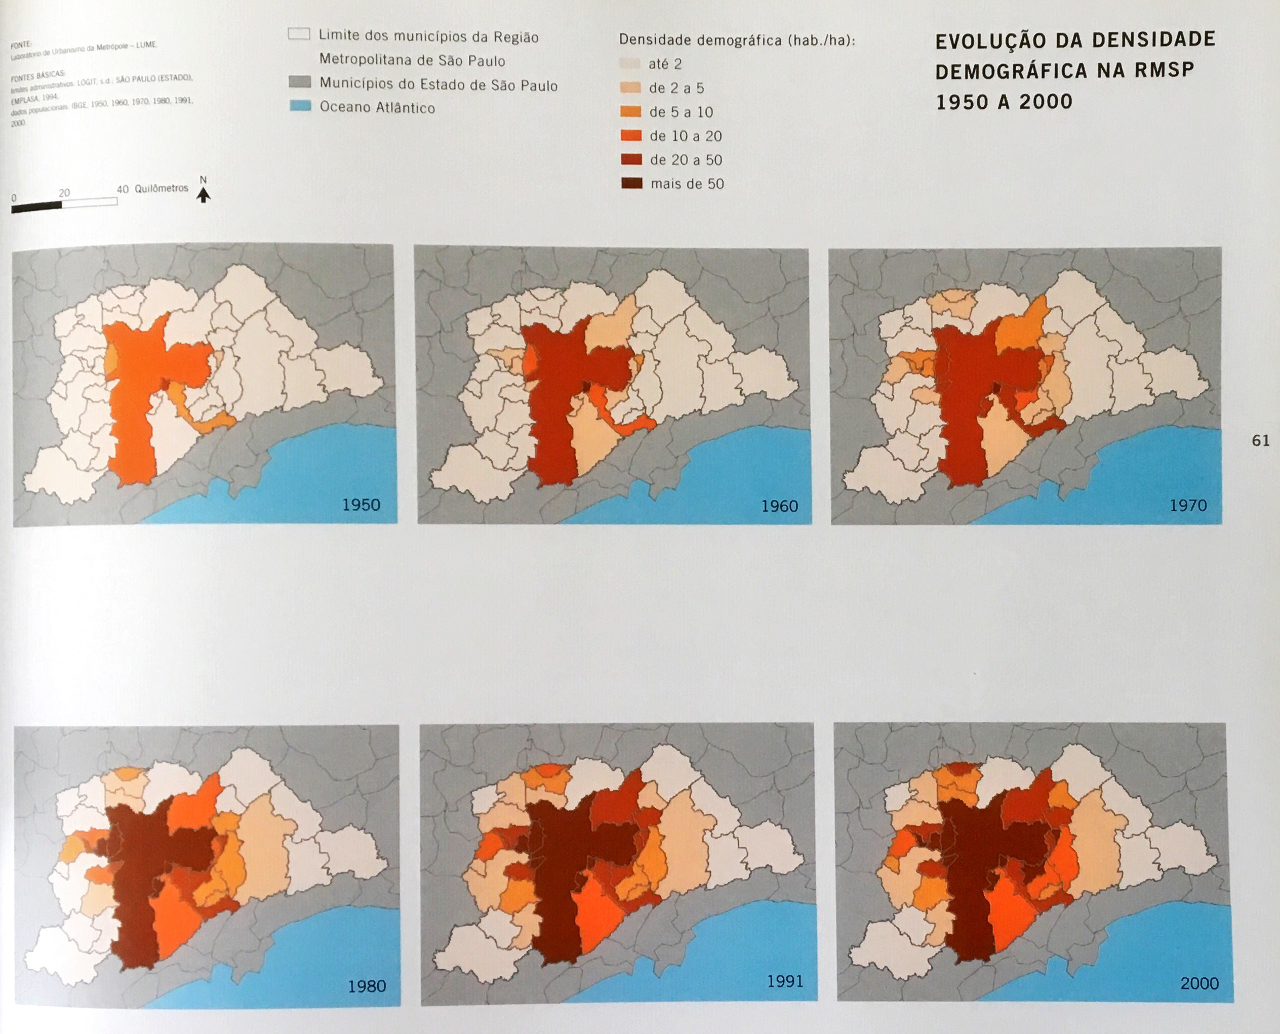
\includegraphics[width=\linewidth,keepaspectratio]{img/spmetrop_pag061}
		\label{spmetrop_pag061}
		\legend{Elaboração por \citeonline[p.61]{meyer2004}}
	\end{figure}
	
	Para compreendermos a situação apontada, \citeonline[p.32]{pasternak2005a} sublinham que, ``em 1991, todos os municípios com taxas de crescimento no período 1980-1991 maiores que 5,5\% a.a. possuíam proporção de migrantes maior que	30\%: Arujá, Barueri, Embu-Guaçu, Francisco Morato, Itapevi, Jandira, Itaquaquecetuba e Santana de Parnaíba''. Consideremos também que ``em 1991, 58,79\% dos migrantes recentes residiam nos municípios periféricos e, em 2000, essa proporção subiu para 61,46\%'' \cite[p.32]{pasternak2005a}. Tal fenômeno pode ser melhor compreendido, ao considerarmos que, ainda que na década de 1980 o panorama do mercado de trabalho tenha sido alterado, traduzindo-se numa queda de redução dos fluxos migratórios para a \gls{rmsp} registrada pelo censo demográfico de 1991, a região continuou se expandindo, mesmo tendo perdido 275 mil habitantes. Para se ter uma ideia do crescimento metropolitano, é oportuno destacar que aproximadamente 875 mil indivíduos se redistribuíram no interior do território \cite[p.42]{meyer2004}.

	\begin{figure}[h]
		\centering
		\caption{Evolução da área urbanizada - 1949-1992}
		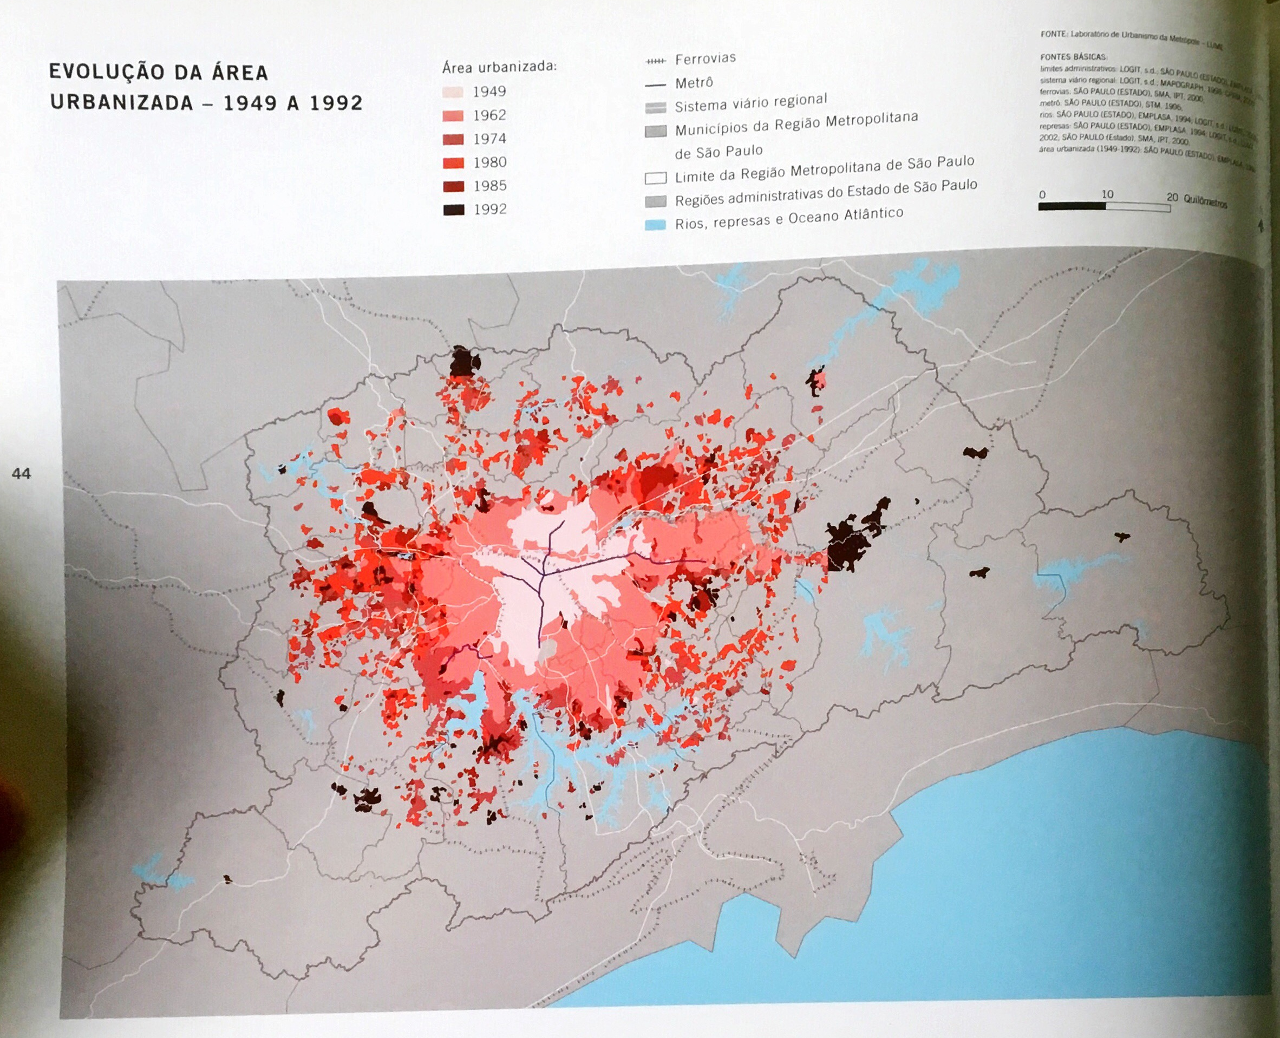
\includegraphics[width=\linewidth,keepaspectratio]{img/spmetrop_pag044}
		\label{spmetrop_pag044}
		\legend{Elaboração por \citeonline[p.44]{meyer2004}}
	\end{figure}
	
	O mapa contido na figura \ref{spmetrop_pag044} sintetiza a evolução da área urbanizada entre 1949 e 1992 e, como pode ser observado neste, Francisco Morato exibiu evolução da área urbanizada sobretudo na tríade 1980-1985-1992. A redistribuição da população também pode ser avaliada no período 2005/2010, vide figura \ref{marques2015_pag134}, na qual revela-se um fluxo migratório entre Francisco Morato e a capital superior a 6 mil pessoas mas inferior a 8 mil pessoas, adicionalmente, \apudonline[p.130]{nobre2010a}{marques2015} aponta que entre 2002 e 2007 houve um incremento de 232 km² nas áreas urbanas da \gls{rmsp}, ainda que a metrópole passasse por um momento de baixo incremento demográfico. Ainda no contexto da figura \ref{marques2015_pag134}, \citeonline[p.135]{marques2015} conclui que ``o município de São Paulo continua sendo o grande `fornecedor' de população para áreas cada vez mais distantes''.
	
	\citeonline[p.131]{nobre2010a} também reforça ``a importância da migração intrametropolitana, não apenas em termos de volume, mas sobretudo pelo seu impacto em vários municípios da região'', apontando ainda que ``a migração com origem nos municípios da \gls{rmsp} constitui parte significativa de migração recebida por essas áreas'', bem como o impacto nos municípios de caráter mais periférico. Para melhor contextualizar o impacto, \citeonline[p.133]{marques2015} identificou ``cifras impressionantes da ordem de 50 mil pessoas/ano se transferindo para as regiões mais periféricas'', o que significa que as propostas para Francisco Morato precisam considerar tal fenômeno, de maneira a reduzir a vulnerabilidade do município e a população que nele já reside, pois como \cite[p.137]{marques2015} salienta:
	
	\begin{citacao}
		``(\dots )sem desconsiderar todos os demais avanços que precisam ser obtidos na área de gestão e políticas públicas, a \gls{rmsp} precisa enfrentar questões essenciais, de forma a permitir um melhor acesso à cidade por parte daquele que poderíamos chamar de `cidadão metropolitano'. Progressos nas áreas de habitação, um zoneamento mais equitativo \textendash influenciado, entre outros aspectos, pela maior regulação do uso do solo por parte do poder público \textendash, atenção prioritária para a mobilidade urbana, que permitira estabelecer o real direito de `ir e vir', entre outros, são temas cruciais para combate e/ou mitigação dos efeitos que a redistribuição da população no espaço tem sobre o dia a dia das pessoas''.
	\end{citacao}
	
	\begin{figure}[h]
		\centering
		\caption{Fluxos migratórios intrametropolitanos superiores a 4,5 mil pessoas na \gls{rmsp} - 2005/2010}
		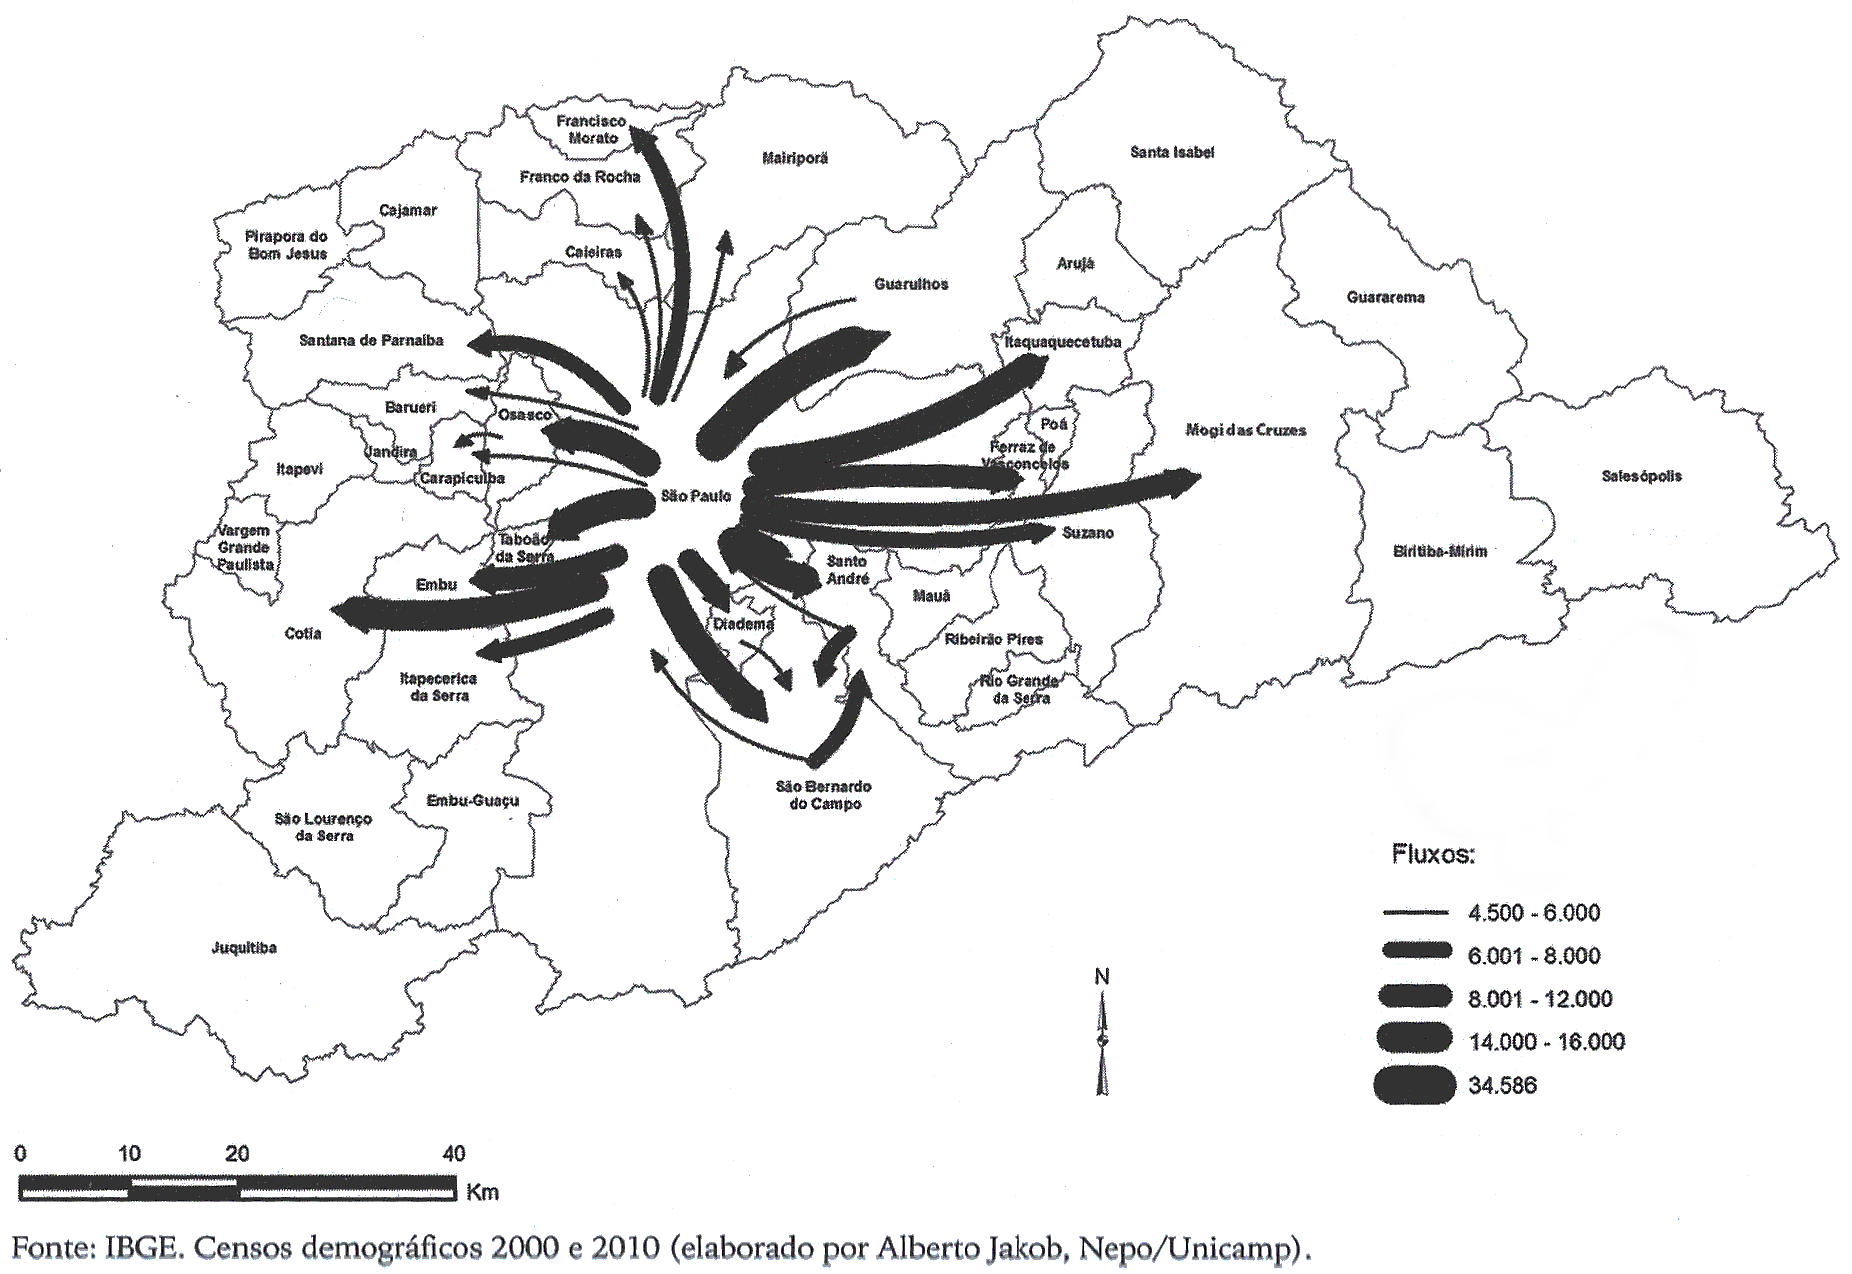
\includegraphics[width=\linewidth,keepaspectratio]{img/marques2015_pag134}
		\label{marques2015_pag134}
		\legend{Reproduzido de \citeonline[p.134]{marques2015}}
	\end{figure}
	
	Realizando uma comparação entre 1970 e 2014, \citeonline[p.19]{cunha2014a} destaca que ``no período de 44 anos as alterações mais significativas, impactantes e intensas se deram em alguns municípios'' e, prossegue: ``Francisco Morato aumentou em 14,8 vezes esse indicador, saindo de 229 habitantes/km² para 3.393 habitantes/km²''.
	
	\subsection{Fragilidade institucional}
	
	Conforme \citeonline[p.59]{cassiele2007a} ``a cidade está inserida em um ciclo de pobreza que barra o desenvolvimento da	mesma, uma vez que a prefeitura não possui estrutura administrativa e financeira para lidar com o constante aumento dessa pobreza e para suprir as novas demandas da população'', que também aponta que mesmo o centro do município ``possui inúmeros problemas de infra-estrutura, o que mostra a precariedade e a incapacidade do poder local para	se mobilizar e buscar alternativas aos problemas da cidade'' \cite[p.61]{cassiele2007a}, bem como que ``os serviços públicos deixam a desejar, em todo o município, quando falamos de saneamento básico e conservação ambiental, principalmente no que se refere à coleta de esgotos que atende apenas 27\% da população, enquanto que a média da RMSP é de 59,7\%'' \cite[p.63]{cassiele2007a}.
	
	\subsection{Fragilidade socioeconômica}
	
	Para \citeonline[p.90]{cassiele2007a}, ``o processo de ocupação do território e crescimento populacional é contínuo, porém as atividades econômicas e fatores que apoiem o desenvolvimento social são escassos ou estagnados; isso aliado à má localização e falta de infra-estrutura faz com que o preço da terra na cidade seja baixo, fato que transformam Francisco Morato em um local atrativo para a concentração de pobreza, como já acontece'', pontuando ainda que ``a precariedade nas condições da estrutura urbana e o baixo índice de desenvolvimento
	social são fatores que, em conjunto com outros determinantes econômicos externos, fazem de Francisco Morato uma cidade economicamente estagnada'' \cite[p.92]{cassiele2007a}, pois ``a falta de emprego na cidade é grande e a industrialização é muito pequena. Sem infra-estrutura a cidade não consegue oferecer vantagens para atrair as empresas ou qualquer outro
	tipo de investimento capitalista privado'' \cite[p.99]{cassiele2007a}.
	
	Finalmente, para \citeonline[p.52]{carvalho2018a}, ``o aprofundamento do processo de redistribuição de renda no Brasil só seria possível, portanto, com uma reforma tributária progressiva que taxasse menos o consumo e a produção e mais a renda e o patrimônio''.
	
	\section{Os traços marcantes da trajetória} \label{sec:tracos-sumario}
	% Item 4 da metodologia adotada:
	% Quais são os traços marcantes (causas) que respondem por esta trajetória do território?
	%
	
	Sumarizando, são os traços marcantes:
	
	\begin{itemize}
		\item Ligação ferroviária entre municípios para escoamento da produção de café (construção da \gls{spr});
		\item Emancipação de Franco da Rocha;
		\item Migração nordestina.
	\end{itemize}
	
	\section{Um breve balanço}
	% Item 2 da metodologia adotada:
	% Esta trajetória é ascendente ou descendente?
	%
		
	Tratou-se de uma trajetória ascendente, pois como vimos na seção \ref{sec:balanco}, ainda que o município apresente índices insatisfatórios de desenvolvimento, este conta com uma ligação sobre trilhos de caráter estratégico e seu território pode ser melhor qualificado para abrigar a população atualmente residente.

	\chapter{O passado encontra o presente e esboça o futuro}
	% Item 5 da metodologia adotada:
	% Em  que  a  etapa  atual  desta  história  difere  da  anterior  e  que  desafios  ela  traz  para  se pensar o futuro do território?
	%
	
	O processo de urbanização da região que atualmente corresponde à área do município de Francisco Morato tem ponto de partida na ampliação da rede de comunicação entre as cidades por meio das linhas ferroviárias.
	
	Nos anos 60, quando ainda era um distrito de Franco da Rocha, boa parte da população era constituída por migrantes nordestinos que foram relegados ao papel de mão de obra barata e de baixa qualificação. Uma abordagem sobre migração pode ser conferida na subseção \ref{CrescimentoMigracao}.
	
	O município tem baixo potencial de atração: ``Francisco Morato e Rio Grande da Serra mantêm-se, entre os municípios servidos pela \gls{cptm}, como os que menos atraem de outros municípios'' \cite[p.80]{ferreira2010a}.
	
	\subsection{Indicadores}
	
	Francisco Morato é o município de menor \gls{idhm} da Região Metropolitana de São Paulo e também está entre as maiores densidades demográficas da região, de 3239,11 hab/km². São incluídos entre os índices o baixíssimo nível educacional e alta taxa de gravidez na adolescência. Esses são alguns dos indicadores dos entraves pelos quais perpassa as possibilidades de desenvolvimento do município.
	
	\subsection{Composição étnica-racial}

	\begin{landscape}
		\begin{figure}[h]
			\centering
			\caption{Mapa racial de Francisco Morato}
			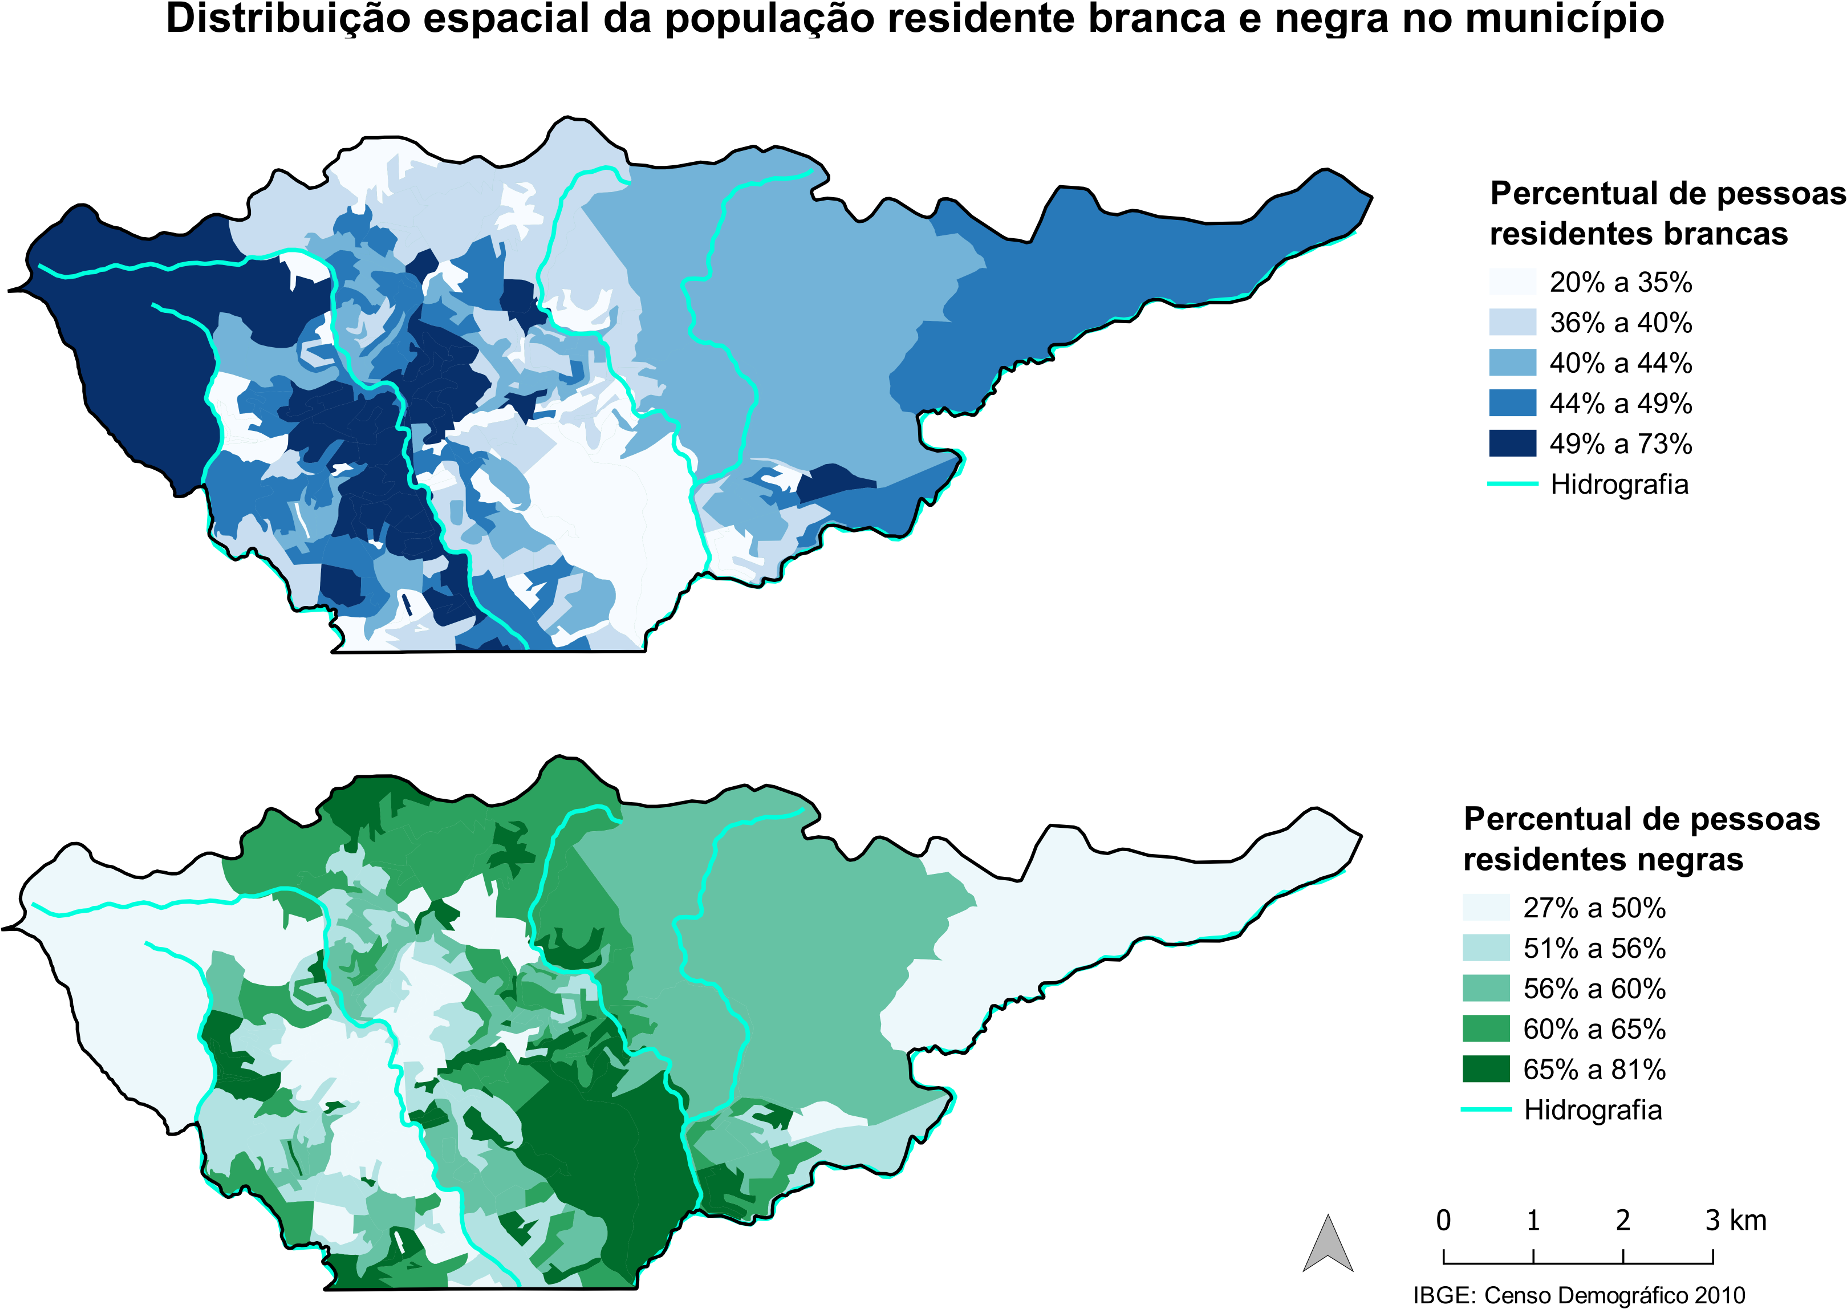
\includegraphics[height=14cm,keepaspectratio]{img/ResidentesNegroseBrancos_BaixaRes.png}
			\label{mapa_racial}
			\legend{Elaboração própria. Fonte: \citeonline{ibge2010a}}
		\end{figure}
	\end{landscape}
	
	\subsection{Mobilidade} \label{Mobilidade}
	
	%TODO Ainda faltam mais coisas para construir um bom parágrafo sobre pendularidade
	\citeonline[p.62]{suarez2014a} aponta que Francisco Morato está entre os municípios que apresentaram ``aumento no número de
	pessoas que realizam movimentos pendulares na primeira década do século XXI'', sendo que, assim como Franco da Rocha e Caieiras, Francisco Morato possui ``cerca de 25\% de sua população realizando movimentos pendulares para outros municípios, com cerca de 62 a 72\% destes deslocamentos com destino a São Paulo'' \cite[p.72]{suarez2014a}.
	
	\begin{figure}[!htb]
		\centering
		\caption[Embarques por estação da Linha 7 - 2010]{Embarques por estação - média dos dias úteis e participação no total de embarques da Linha 7 – 2010}
		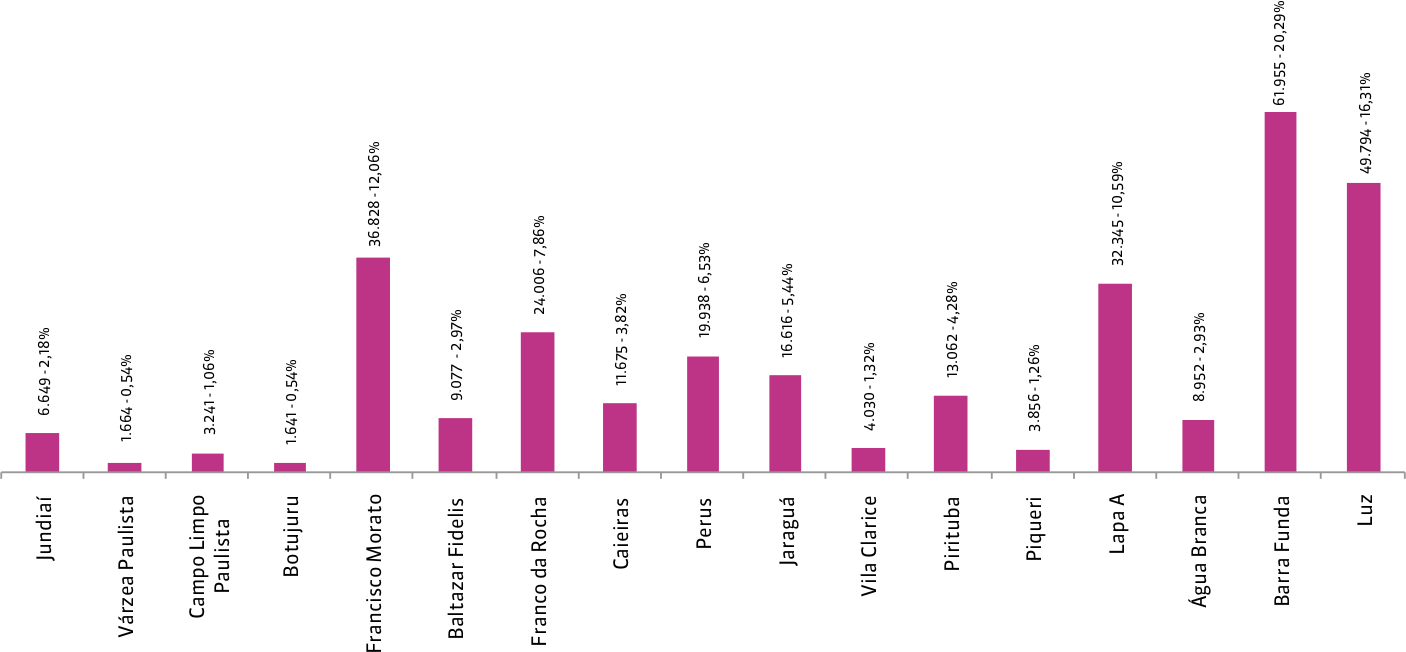
\includegraphics[width=\linewidth]{img/pdcptm_57a}
		\label{fig:pdcptm_57a}
		\legend{Fonte: \citeonline[p.57]{cptm2010a}}
	\end{figure}
    
    A presença da Linha 7-Rubi é um elemento marcante da mobilidade moratense, cujas consequências de sua ausência podem ser observadas no levantamento realizado por \cite[p.32-33]{ferreira2010a}, que sumariza o quadro após o fechamento da linha em 1996, fruto de depredações pela população como forma de manifestação da insatisfação com a qualidade dos serviços.
    
    \begin{citacao}
    	Na ocasião, cerca de meio milhão de moradores da região ficaram sem o trem e tiveram que se reorganizar para conseguir se locomover. Estimou-se na época que uma frota de 230 novos ônibus, entre clandestinos e reservas da São Paulo Transportes (SPTRANS), foram colocados nas ruas para tentar solucionar o transporte de quem dependia exclusivamente do trem. Além disso, outras 200 lotações ocuparam as ruas próximas às estações paralisadas, concorrendo pelos novos passageiros. Algumas consequências podem ser destacadas:
    	
    	\begin{itemize}[leftmargin=\leftskip+\labelwidth-\labelsep]
    		\item Acréscimo no desembolso dos usuários para se locomover, que em alguns locais
    	passou de R\$ 0,80 para R\$ 2,00 por viagem, nas lotações;
	    	\item Acréscimo do tempo de viagem, adicionando até duas horas a mais com filas e no
    	percurso, que, com o trem, era feito em 40 minutos;
	    	\item Aumento dos congestionamentos da Av. Raimundo Pereira Magalhães e demais vias
    	que dão acesso às cidades de Caieiras e Francisco Morato, devido à falta de infra-
    	estrutura necessária ao acréscimo de 35\% do movimento;
		    \item Aumento de acidentes da ordem de 20\% em algumas rodovias. A maior causa foi o
    	desgaste do pavimento e aumento dos buracos.
		\end{itemize}
    \end{citacao}
    
    \citeonline[p.33]{ferreira2010a} também aponta ``queda nas vendas de até 85\% em cidades como Francisco Morato e Caieiras, somando dezenas de lojas e galerias falidas, 29 mil desempregados na região, além de outros milhares que não conseguiram empregos pela falta de locomoção'', salientando a crucialidade do funcionamento do transporte ferroviário metropolitano para a sustentação do comércio e do modo de vida dos habitantes.
    
    Destaca-se também a alteração no formato de operação da Linha 7-Rubi, nascida não apenas com a incorporação da Linha Noroeste-Sudeste da \gls{cbtu}, mas com a separação desta em duas linhas distintas \cite[p.50]{ferreira2010a} \cite[p.223]{stefani2007a}.

	\begin{figure}[H]
		\centering
		\caption{Vias de acesso para Francisco Morato}
		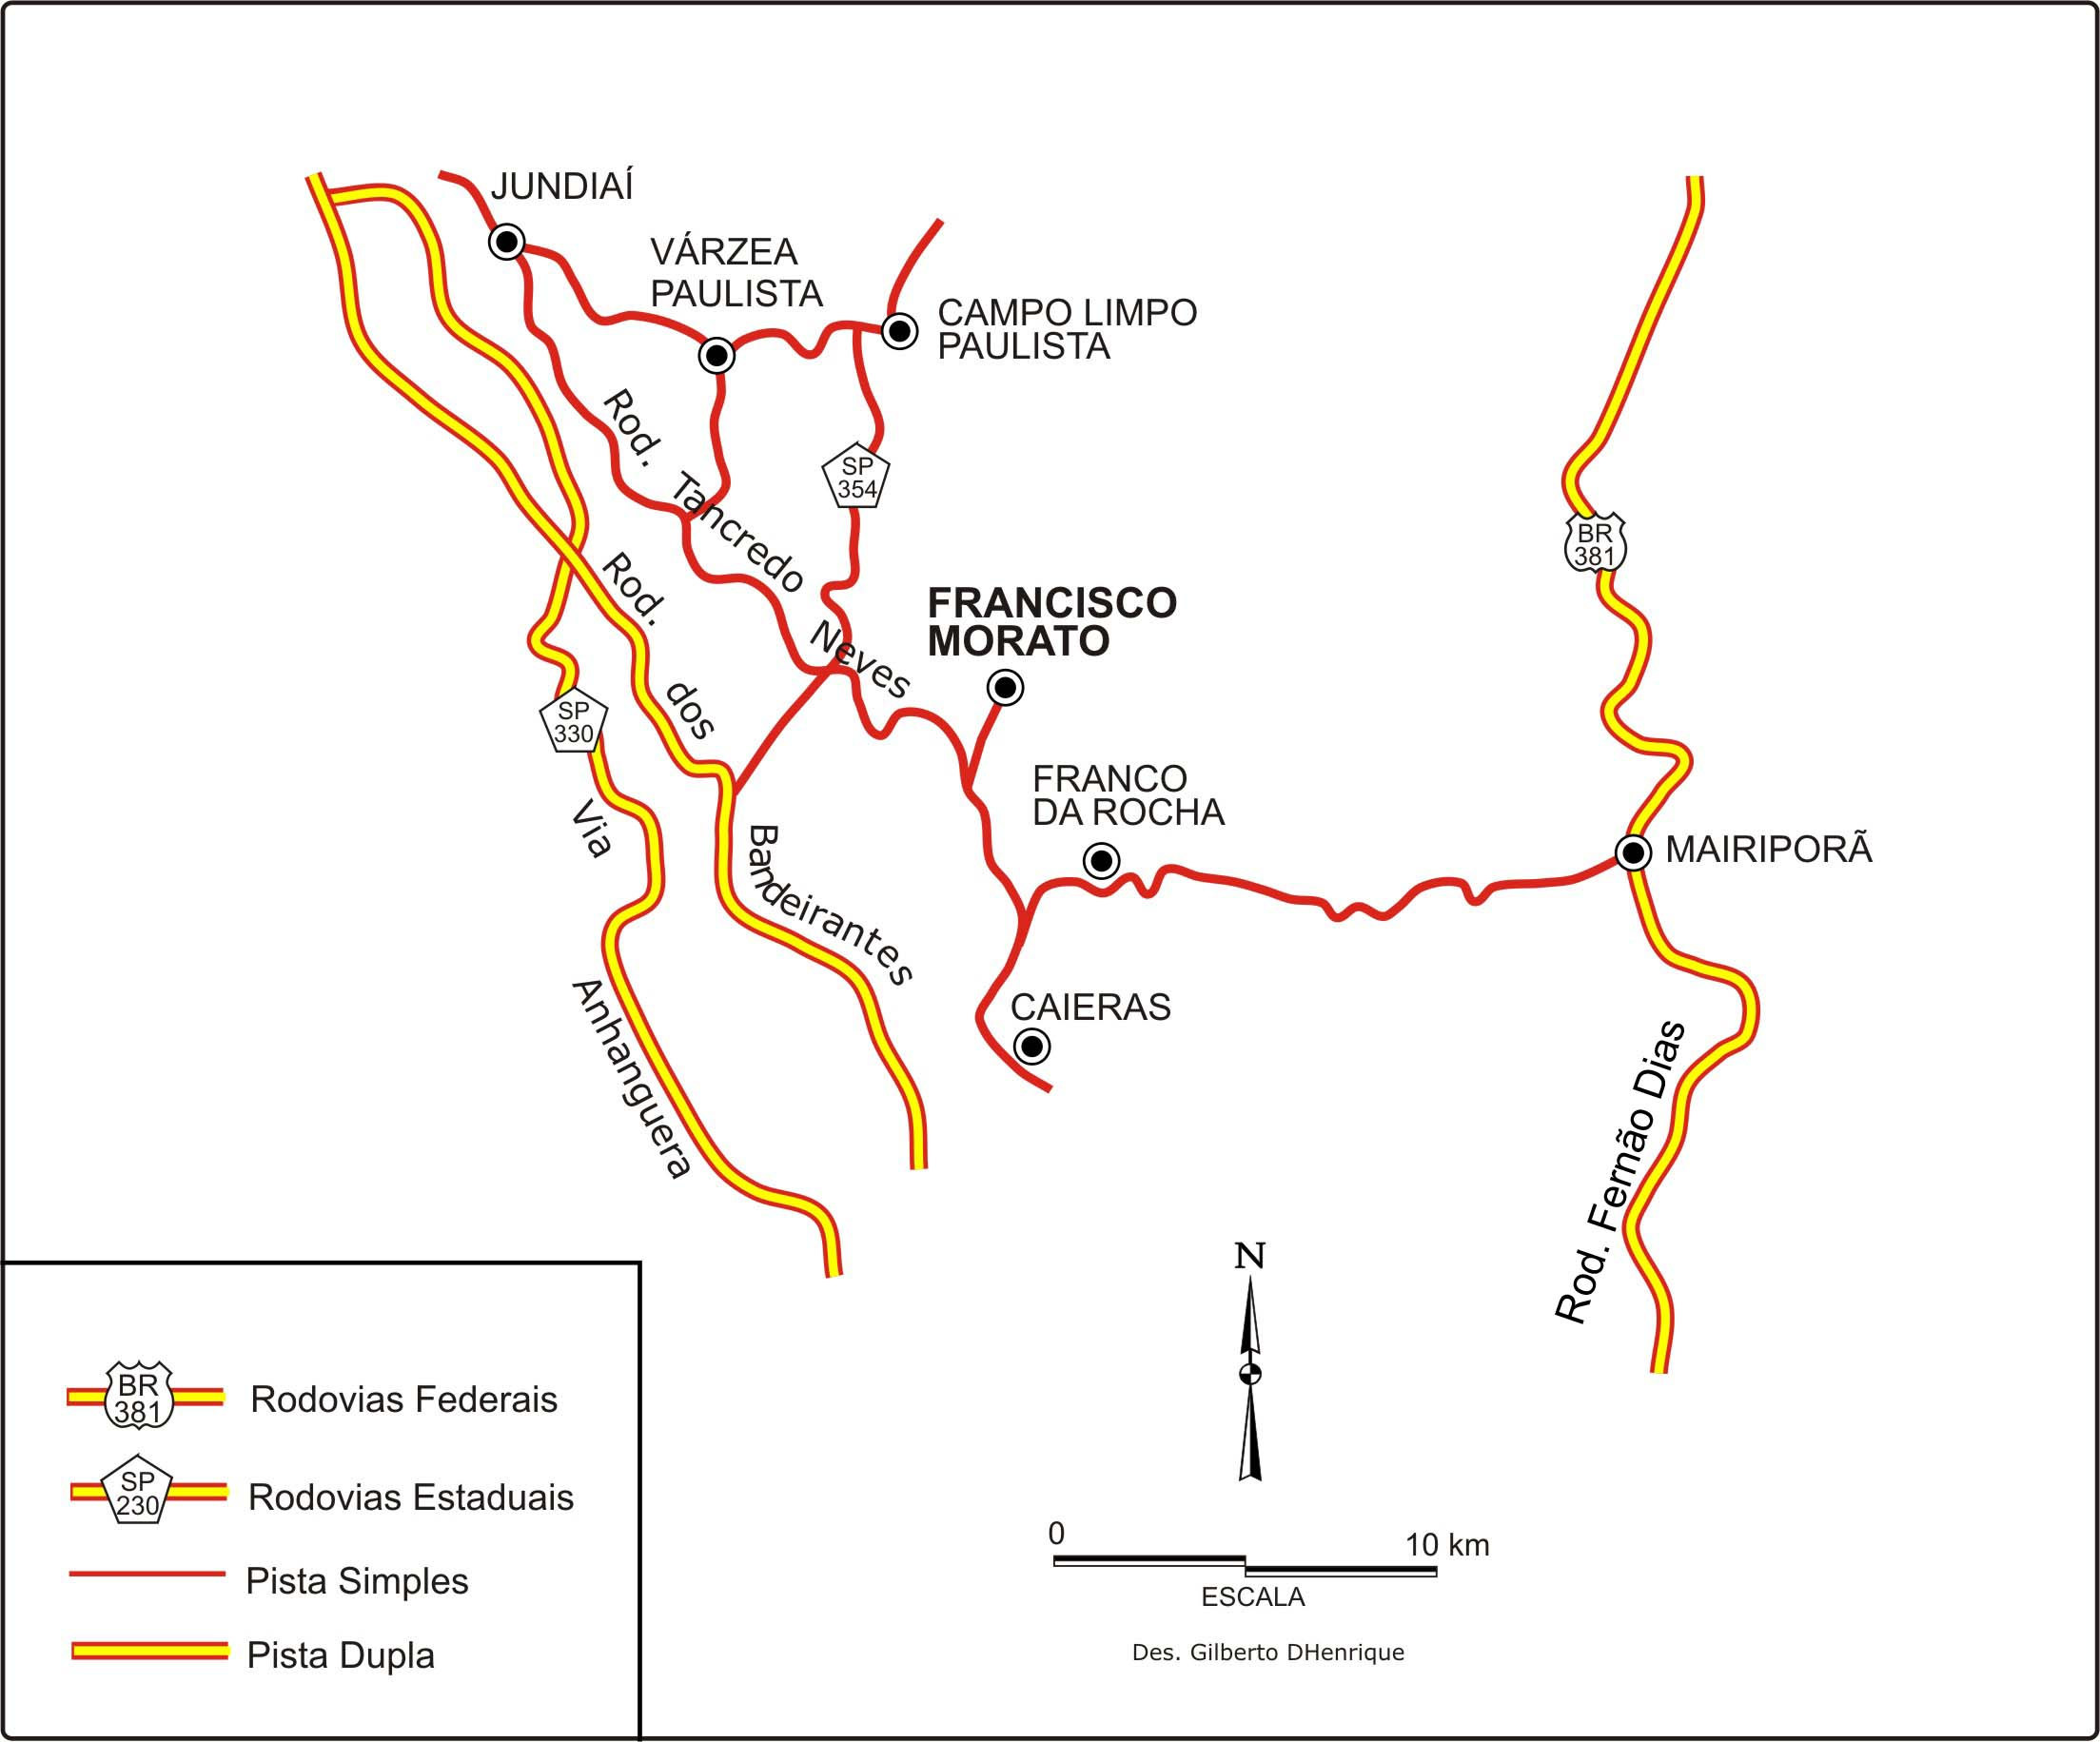
\includegraphics[height=8cm]{img/cassiele_vias_acesso}
		\label{fig:vias_acesso}
		\legend{Fonte: \citeonline[p.88]{cassiele2007a}}
	\end{figure}
    
    Quanto ao transporte rodoviário, ``a Rodovia Tancredo Neves (SP 332), também ficou imersa na mancha urbana, assumindo uma característica de via urbana, e ligando a cidade de São Paulo à Caieiras, Franco da Rocha e Francisco Morato indo até Jundiaí'' \cite[p.49]{suarez2014a}.
	
	Para \citeonline[p.89]{cassiele2007a}, considerando a relação entre Francisco Morato e os municípios de São Paulo, Franco da Rocha, Caieiras e Campo	Limpo Paulista, ``a precariedade e insuficiência de acesso via estradas entre Francisco Morato e essas cidades prejudica o desenvolvimento econômico deste município. Já é sabido que lugares sem acesso por estradas e rodovias não são atraentes para investimentos empresariais, uma vez que há grande dificuldade de escoamento e circulação da produção''.
	
	\begin{figure}[h]
		\centering
		\caption{Estrutura viária e de transportes metropolitana}
		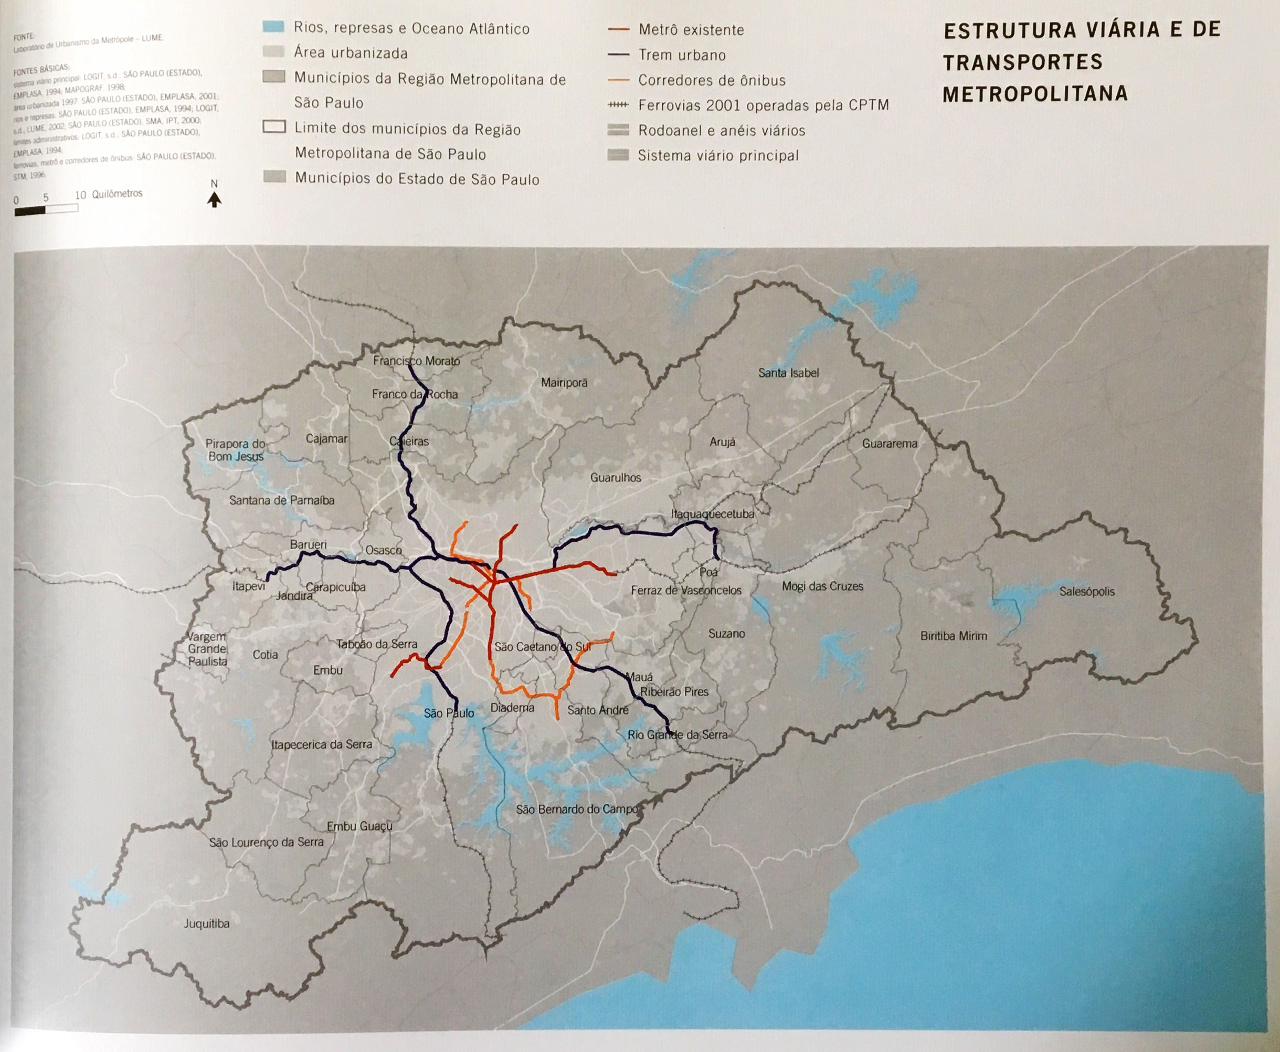
\includegraphics[width=\linewidth,keepaspectratio]{img/spmetrop_pag075}
		\label{spmetrop_pag075}
		\legend{Elaboração por \citeonline[p.75]{meyer2004}}
	\end{figure}	
	
	\subsection{Saneamento Básico}
	
    Dados de 2016 do \glsdesc{snis} indicam que apenas 40\% da população urbana é atendida por esgotamento sanitário. Ainda, de acordo com o relatório do Plano de Bacia Hidrográfica do Alto Tietê, elaborado pela \gls{fabhat}, o esgoto é integralmente lançado \textit{in natura} em corpos d'água.
    
   	\begin{center}
   		\begin{longtable}{p{1cm} p{3cm} p{3cm} p{3cm} p{3cm}}
   			\caption{Renda e infraestrutura em Francisco Morato em 1991 e 2000} \label{tab_spmetro_pag100}\\
   			\hline
   			\textbf{Ano} & \textbf{porcentagem de domicílios com renda do chefe até 1 salário mínimo, inclusive sem renda} & \textbf{porcentagem de domicílios ligados à rede pública de água com canalização interna} & \textbf{porcentagem de domicílios ligados à rede pública de esgoto com canalização interna} & \textbf{porcentagem de domicílios com coleta de lixo domiciliar ou com caçamba} \\
   			\hline
   			\endfirsthead
   			\multicolumn{5}{c}%
   			{\tablename\ \thetable\ -- \textit{Continuado da página anterior}} \\
   			\hline
   			\textbf{Ano} & \textbf{porcentagem de domicílios com renda do chefe até 1 salário mínimo, inclusive sem renda} & \textbf{porcentagem de domicílios ligados à rede pública de água com canalização interna} & \textbf{porcentagem de domicílios ligados à rede pública de esgoto com canalização interna} & \textbf{porcentagem de domicílios com coleta de lixo domiciliar ou com caçamba} \\
   			\hline
   			\endhead
   			\hline \multicolumn{5}{r}{\textit{Continua na próxima página}} \\
   			\endfoot
   			\hline
   			\endlastfoot
   			1991 & 10,66\% & 69,13\% & 16,30\% & 33,13\% \\
   			2000 & 31,44\% & 90,66\% & 26,83\% & 83,40\% \\
   		\end{longtable}
   		\legend{Elaboração própria. Fonte: \citeonline[p.100-101]{meyer2004}}
   	\end{center}
   	
   	Com base na tabela acima e nos dados do \gls{snis}, podemos concluir que a evolução da situação do esgotamento sanitário foi insatisfatória na última década e meia, evoluindo aproximadamente 13,17\%.
    
    \subsection{Restrições à ocupação}
    
    Um dos grandes fatores para a manutenção do ciclo de pobreza no município é a grande limitação geológica que o caracteriza. Devido ao relevo formado predominantemente por escarpas, serras e morrotes, os habitantes enfrentam grandes desafios em construir suas casas e consideráveis riscos em mantê-las. 

    De acordo com a Cartas de Suscetibilidade a Movimentos de Massa elaborada pelo \gls{ipt}, as áreas que se enquadram nas categorias de alta e média suscetibilidade a deslizamento correspondem a cerca de 32\% da área urbanizada do município.
    
    Do ponto de vista da paisagem e dos usos do solo, o município apresenta áreas relativamente homogêneas com características distintas entre si. A centralidade que envolve a estação ferroviária e principais vias é caracterizada por alto grau de adensamento e uso misto. É também a região mais favorável à ocupação, visto que é formada predominantemente de morros baixos e apresenta menores riscos de deslizamento e inundação em comparação com o restante do município. 
    
    O aumento na declividade e a transição para relevo de morros altos que qualificam a parcela norte do município são acompanhados de um decréscimo na densidade populacional. O mesmo ocorre com extremidade esquerda da cidade, que faz limite com os municípios de Franco da Rocha e Campo Limpo Paulista. Caracterizada por serras e escarpas, altas declividades, a região possui alta suscetibilidade a deslizamento, fazendo com que existam apenas algumas ocupações pontuais \textendash grande parte em área de risco. A faixa sudeste, limítrofe com o município de Mairiporã, abriga o bairro Jardim Alegria e possui características de ocupação singulares. O Jardim Alegria é uma ocupação irregular consolidada em região de morros baixos, envolta por planícies fluviais de alta suscetibilidade a inundação. 
    
    Para além das centralidades com alta densidade populacional que acompanham o eixo ferroviário e a ocupação do Jardim Alegria, a parcela central a nordeste do município apresenta ocupações pontuais e muito dispersas, grande taxa de vegetação e pequenos focos de vegetação nativa. A extremidade à direita, também limítrofes com os municípios de Atibaia, Mairiporã e Franco da Rocha é caracterizada por baixíssima densidade populacional. Além disso, essa região concentra as propriedades rurais do município. 

    \begin{figure}[ht]
		\centering
		\caption{Suscetibilidade a movimento de massa e áreas ocupadas}
		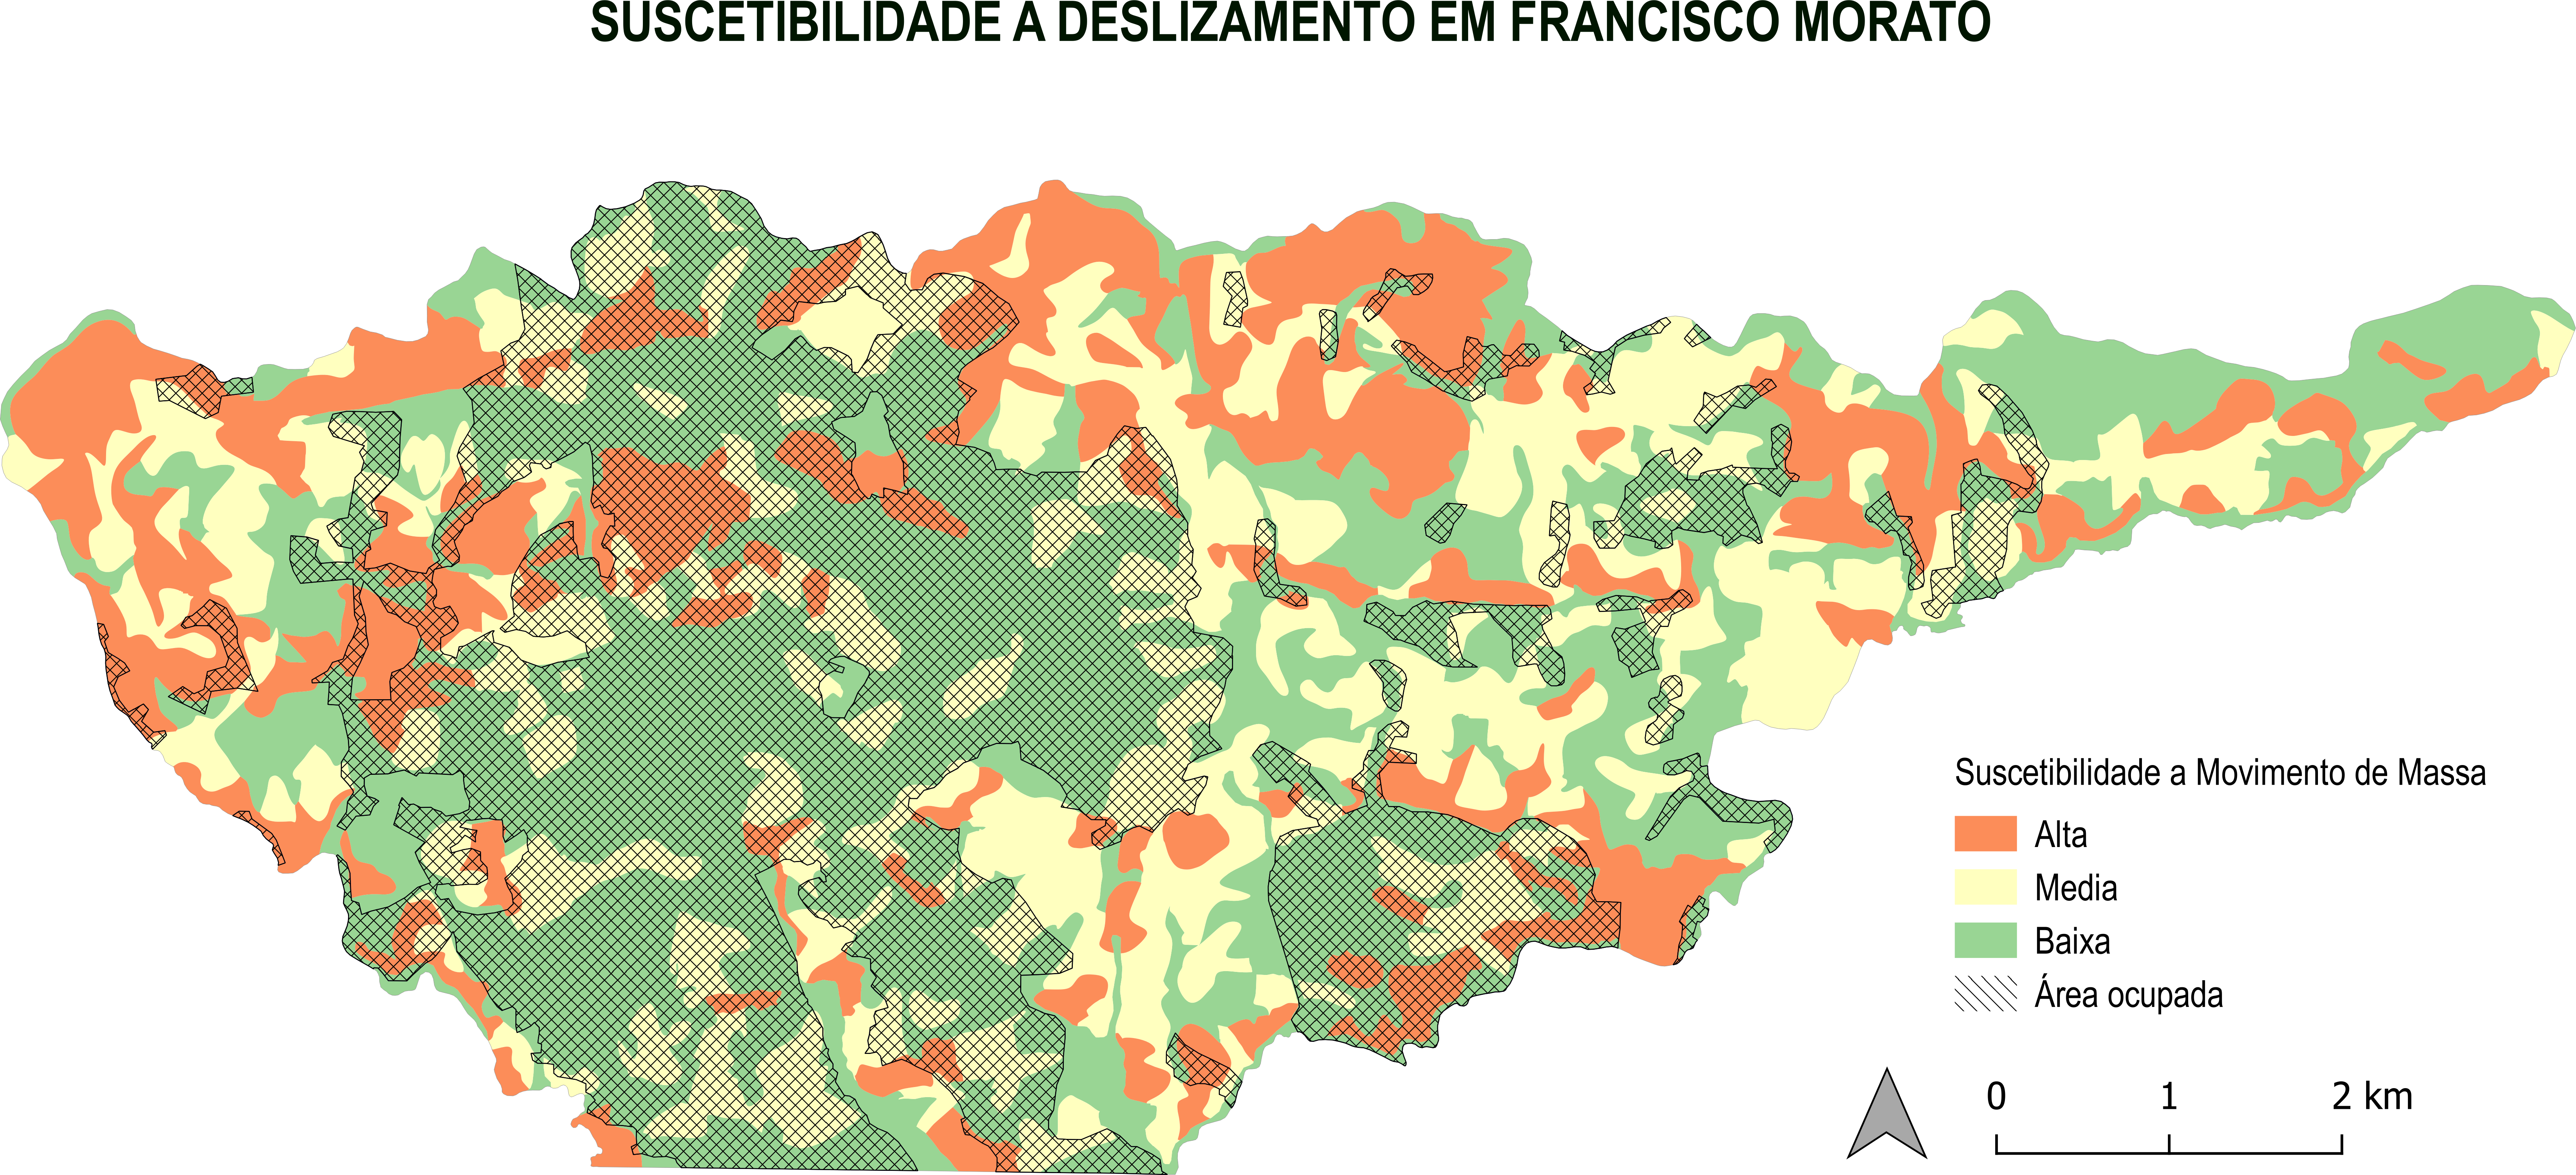
\includegraphics[width=\linewidth]{img/DESLIZAMENTOF5_BaixaRes.png}
		\label{fig:movimento_massa}
		\legend{Elaboração própria. Fonte: Limites municipais \cite{cem2015a} e Carta de Suscetibilidade de Franscisco Morato \cite{cprm2015a}}
	
		\caption{Suscetibilidade a inundação e proposta de área de preservação permanente}
		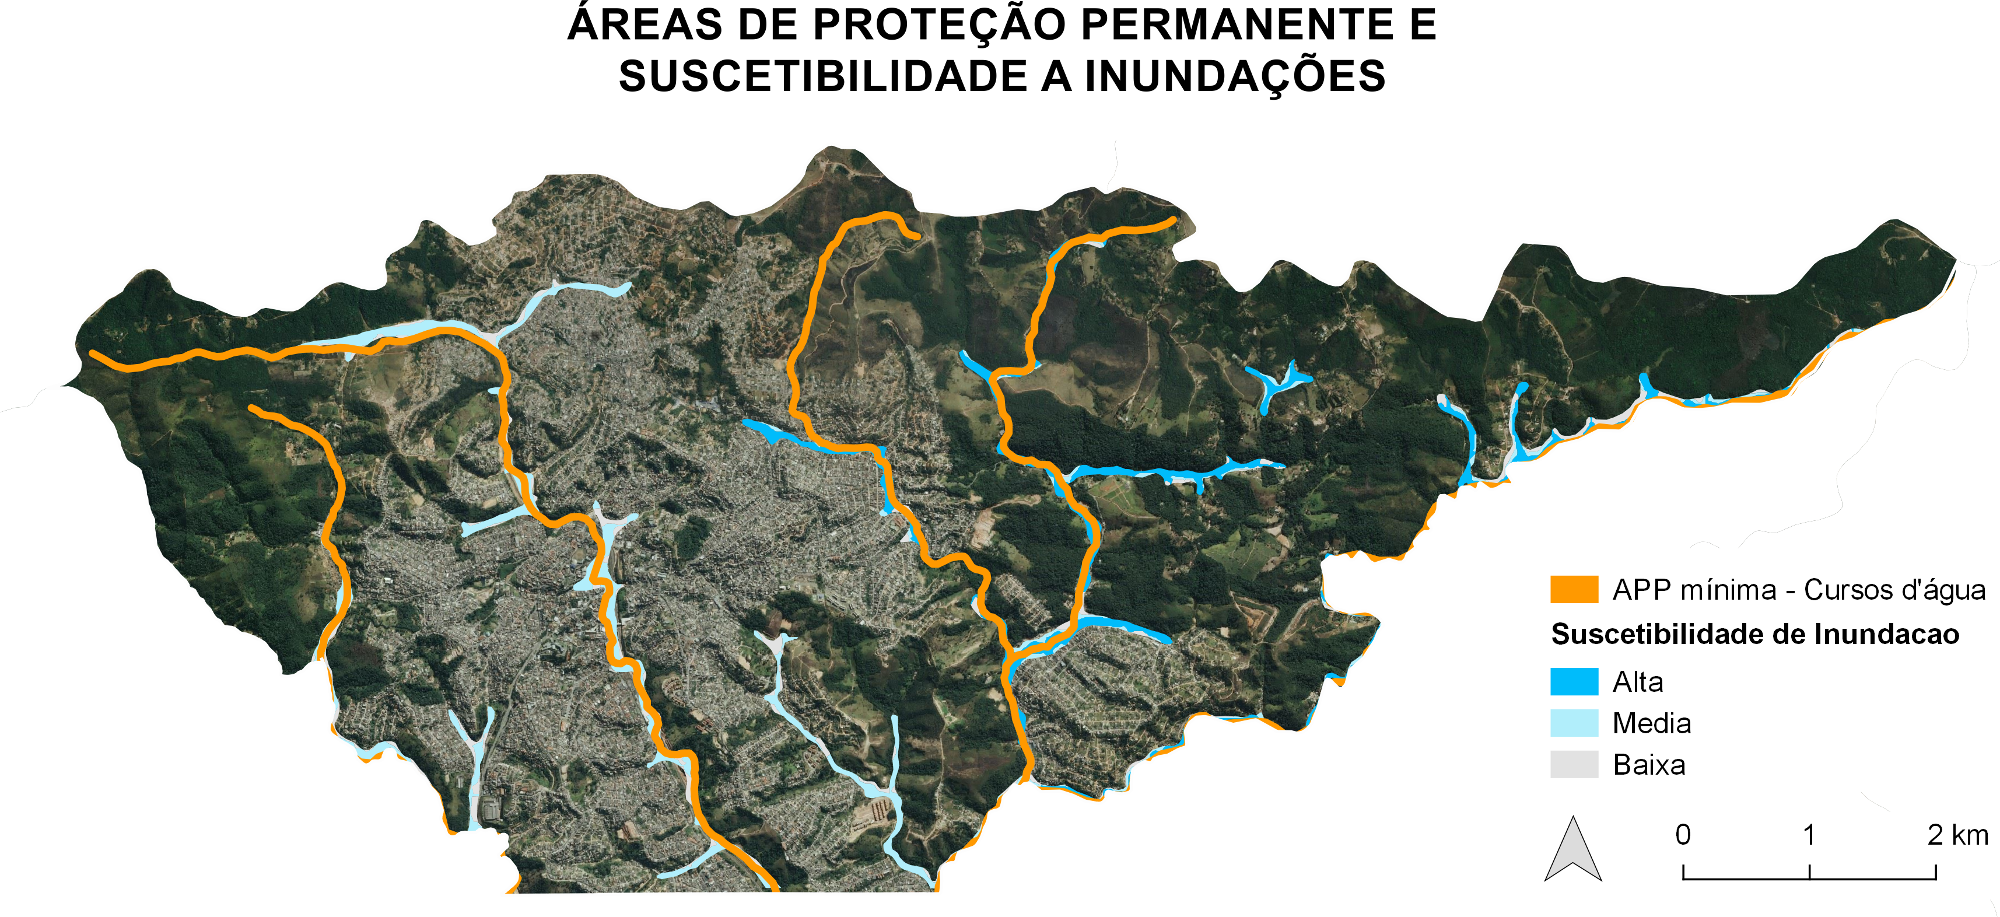
\includegraphics[width=\linewidth]{img/APPeInundacao2_BaixaRes.png}
		\label{fig:inundacao}
		\legend{Elaboração própria. Fonte: Hidrografia \cite{cem2015a} e Carta de Suscetibilidade de Franscisco Morato \cite{cprm2015a}}
	\end{figure}

	Sabendo-se que ``em vinte anos, desde 1971, o processo de urbanização destruiu 31\% das áreas recobertas por matas, ocupou fundos de vale com avenidas e favelas, destruiu morros e avançou sobre encostas íngremes e áreas de proteção aos mananciais de abastecimento público'' \cite[p.45]{meyer2004}, o quadro acima descrito não constitui uma surpresa, no entanto, como parte do diagnóstico, que embasará nossas propostas, fica flagrante a necessidade de minorar os efeitos da urbanização, sobretudo em Francisco Morato.

%===============================================================================
%

	% ----------------------------------------------------------
	% ----------------------------------------------------------
	\postextual
	
	
	
	% informa o arquivo com a bibliografia. Deve ser o mesmo nome
	% (sem o sufixo) que será informado no ambiente filecontents
	% que está no final deste arquivo. Neste exemplo foi usado 
	% bibitemp.bib e bibtemp. Este comando insere a bibliografia
	% nesta posição (antes dos apêndices, anexos, índice remissivo)
	\bibliography{fontes}
	% ----------------------------------------------------------
	% Glossário
	% ----------------------------------------------------------
	% Consultar manual da classe abntex2 para orientações sobre o
	% uso do glossário.
	\renewcommand{\glossaryname}{Glossário}
	%\renewcommand{\glossarypreamble}{Esta é a descrição do glossário.\\ \\}
	\renewcommand*{\glsseeformat}[3][\seename]{\textit{#1}
		\glsseelist{#2}}
	
	% ---
	% Traduções para o ambiente glossaries
	% ---
	\providetranslation{Glossary}{Glossário}
	\providetranslation{Acronyms}{Siglas}
	\providetranslation{Notation (glossaries)}{Notação}
	\providetranslation{Description (glossaries)}{Descrição}
	\providetranslation{Symbol (glossaries)}{Símbolo}
	\providetranslation{Page List (glossaries)}{Lista de Páginas}
	\providetranslation{Symbols (glossaries)}{Símbolos}
	\providetranslation{Numbers (glossaries)}{Números} 
	% ---
	
	% ---
	% Imprime o glossário
	% ---
	\cleardoublepage
	\phantomsection
	\addcontentsline{toc}{chapter}{\glossaryname}
	% \glossarystyle{index}
	% \glossarystyle{altlisthypergroup}
	\glossarystyle{tree}
	\printglossaries
	% ---
	
	% ----------------------------------------------------------
	% Apêndices
	% ----------------------------------------------------------
	
	% ---
	% Inicia os apêndices. Não esquecer de fechar ao final de
	% todos os apêndices (\end{apendicesenv})
	% ---
	%\begin{apendicesenv}
	
	% Imprime uma página indicando o início dos apêndices
	%\partapendices
	
	% ----------------------------------------------------------
	%\chapter{Primeiro apêndice}
	% ----------------------------------------------------------
	
	%Este é um exemplo de inclusão de capítulos de %apêndice em uma 
	%monografia.  Cada apêndice é tratado como se fosse %um capítulo.
	%Os apêndices devem ser iniciados pelo comando de %ambiente
	%\textbackslash begin\{apendicesenv\} e encerrados %pelo comando 
	%\textbackslash end\{apendicesenv\}.
	
	% ----------------------------------------------------------
	%\chapter{Segundo apêndice}
	% ----------------------------------------------------------
	
	%Este é um exemplo de inclusão de um segundo apêndice. 
	
	%\end{apendicesenv}
	% ---
	
	
	% ----------------------------------------------------------
	% Anexos
	% ----------------------------------------------------------
	
	% ---
	% Inicia os anexos
	% ---
	%\begin{anexosenv}
	
	% Imprime uma página indicando o início dos anexos
	%\partanexos
	
	% ---
	%\chapter{Anexo I}
	% ---
	%Os anexos são similares aos apêndices se distinguindo pelo fato
	%que os apêndices são de autoria do autor da monografia e os 
	%anexos não são da autoria do autor da monografia.  Por exemplo,
	%se incluir no trabalho um modelo de um formulário preenchido
	%por alunos participantes de uma pesquisa, este será um apêndice
	%se o formulário foi criado pelo autor da monografia e será um
	%anexo se o formulário tiver sido criado por outros (por exemplo,
	%é um formulário padrão da escola em que o aluno que o preenche
	%estuda).
	%
	%Mesmo que o formulário tenha sido elaborado pela escola, uma
	%reprodução do formulário preenchido por cada aluno na pesquisa
	%será incluído no apêndice pois envolve o trabalho do autor da
	%monografia ao distribuir, coletar e reproduzir as respostas.
	%
	%Este é um exemplo de inclusão de capítulos de anexos em uma 
	%monografia.  Cada anexo é tratado como se fosse um capítulo.
	%Os anexos devem ser iniciados pelo comando de ambiente
	%\textbackslash begin\{anexoenv\} e encerrados pelo comando 
	%\textbackslash end\{anexoenv\}.
	%
	%\end{anexosenv}
	% ---
	%---------------------------------------------------------------------
	%---------------------------------------------------------------------
	
	%\printindex
	
	% Por padrão são incluídas no trabalho somente as referências
	% citadas ao longo do texto. No comando abaixo foram acrescentadas
	% algumas referências não citadas (neste texto servem apenas como
	% exemplos). Não deve ser usado o comando (mais simples) 
	% \nocite{*}, pois este parece não ser compatível com o
	% abntex2cite
	%\nocite{abntex2cite,abntex2wiki,boyer,eves,iezzi,kletenic,
	%        diomara,steinbruch,intusolatex,feynman,shannon,
	%        luisfelipe,turing}
\end{document}
